\documentclass[twoside]{book}

% Packages required by doxygen
\usepackage{fixltx2e}
\usepackage{calc}
\usepackage{doxygen}
\usepackage[export]{adjustbox} % also loads graphicx
\usepackage{graphicx}
\usepackage[utf8]{inputenc}
\usepackage{makeidx}
\usepackage{multicol}
\usepackage{multirow}
\PassOptionsToPackage{warn}{textcomp}
\usepackage{textcomp}
\usepackage[nointegrals]{wasysym}
\usepackage[table]{xcolor}

% Font selection
\usepackage[T1]{fontenc}
\usepackage[scaled=.90]{helvet}
\usepackage{courier}
\usepackage{amssymb}
\usepackage{sectsty}
\renewcommand{\familydefault}{\sfdefault}
\allsectionsfont{%
  \fontseries{bc}\selectfont%
  \color{darkgray}%
}
\renewcommand{\DoxyLabelFont}{%
  \fontseries{bc}\selectfont%
  \color{darkgray}%
}
\newcommand{\+}{\discretionary{\mbox{\scriptsize$\hookleftarrow$}}{}{}}

% Page & text layout
\usepackage{geometry}
\geometry{%
  a4paper,%
  top=2.5cm,%
  bottom=2.5cm,%
  left=2.5cm,%
  right=2.5cm%
}
\tolerance=750
\hfuzz=15pt
\hbadness=750
\setlength{\emergencystretch}{15pt}
\setlength{\parindent}{0cm}
\setlength{\parskip}{3ex plus 2ex minus 2ex}
\makeatletter
\renewcommand{\paragraph}{%
  \@startsection{paragraph}{4}{0ex}{-1.0ex}{1.0ex}{%
    \normalfont\normalsize\bfseries\SS@parafont%
  }%
}
\renewcommand{\subparagraph}{%
  \@startsection{subparagraph}{5}{0ex}{-1.0ex}{1.0ex}{%
    \normalfont\normalsize\bfseries\SS@subparafont%
  }%
}
\makeatother

% Headers & footers
\usepackage{fancyhdr}
\pagestyle{fancyplain}
\fancyhead[LE]{\fancyplain{}{\bfseries\thepage}}
\fancyhead[CE]{\fancyplain{}{}}
\fancyhead[RE]{\fancyplain{}{\bfseries\leftmark}}
\fancyhead[LO]{\fancyplain{}{\bfseries\rightmark}}
\fancyhead[CO]{\fancyplain{}{}}
\fancyhead[RO]{\fancyplain{}{\bfseries\thepage}}
\fancyfoot[LE]{\fancyplain{}{}}
\fancyfoot[CE]{\fancyplain{}{}}
\fancyfoot[RE]{\fancyplain{}{\bfseries\scriptsize Generated by Doxygen }}
\fancyfoot[LO]{\fancyplain{}{\bfseries\scriptsize Generated by Doxygen }}
\fancyfoot[CO]{\fancyplain{}{}}
\fancyfoot[RO]{\fancyplain{}{}}
\renewcommand{\footrulewidth}{0.4pt}
\renewcommand{\chaptermark}[1]{%
  \markboth{#1}{}%
}
\renewcommand{\sectionmark}[1]{%
  \markright{\thesection\ #1}%
}

% Indices & bibliography
\usepackage{natbib}
\usepackage[titles]{tocloft}
\setcounter{tocdepth}{3}
\setcounter{secnumdepth}{5}
\makeindex

% Hyperlinks (required, but should be loaded last)
\usepackage{ifpdf}
\ifpdf
  \usepackage[pdftex,pagebackref=true]{hyperref}
\else
  \usepackage[ps2pdf,pagebackref=true]{hyperref}
\fi
\hypersetup{%
  colorlinks=true,%
  linkcolor=blue,%
  citecolor=blue,%
  unicode%
}

% Custom commands
\newcommand{\clearemptydoublepage}{%
  \newpage{\pagestyle{empty}\cleardoublepage}%
}

\usepackage{caption}
\captionsetup{labelsep=space,justification=centering,font={bf},singlelinecheck=off,skip=4pt,position=top}

%===== C O N T E N T S =====

\begin{document}

% Titlepage & ToC
\hypersetup{pageanchor=false,
             bookmarksnumbered=true,
             pdfencoding=unicode
            }
\pagenumbering{alph}
\begin{titlepage}
\vspace*{7cm}
\begin{center}%
{\Large Co\+AP Protobuf R\+PC library \\[1ex]\large 0.\+0.\+1 }\\
\vspace*{1cm}
{\large Generated by Doxygen 1.8.13}\\
\end{center}
\end{titlepage}
\clearemptydoublepage
\pagenumbering{roman}
\tableofcontents
\clearemptydoublepage
\pagenumbering{arabic}
\hypersetup{pageanchor=true}

%--- Begin generated contents ---
\chapter{L\+I\+C\+E\+N\+SE}
\label{md_LICENSE}
\Hypertarget{md_LICENSE}
The M\+IT License (M\+IT)

Copyright © 2018 sajanshakya129 Permission is hereby granted, free of charge, to any person obtaining a copy of this software and associated documentation files (the “\+Software”), to deal in the Software without restriction, including without limitation the rights to use, copy, modify, merge, publish, distribute, sublicense, and/or sell copies of the Software, and to permit persons to whom the Software is furnished to do so, subject to the following conditions\+:

The above copyright notice and this permission notice shall be included in all copies or substantial portions of the Software.

The Software is provided “as is”, without warranty of any kind, express or implied, including but not limited to the warranties of merchantability, fitness for a particular purpose and noninfringement. In no event shall the authors or copyright holders be liable for any claim, damages or other liability, whether in an action of contract, tort or otherwise, arising from, out of or in connection with the software or the use or other dealings in the Software. 
\chapter{Protobuf R\+PC over Co\+AP protocol(U\+DP)}
\label{md_README}
\Hypertarget{md_README}
This library is developed to create a R\+PC that utilises features of Co\+AP protocol which uses U\+DP for transport. Protobuf is used as Interface Definition language(\+I\+D\+L). The goal is to use this R\+PC library over Constrained IoT devices.

\subsection*{Getting Started}

The following steps are written with the consideration that the system for development is fresh newly installed Linux Based System.

\subsubsection*{Prerequisites}

Please install following applications to build and install coappbrpc. 
\begin{DoxyCode}
sudo apt-get install cmake build-essential dh-autoreconf python python-pip
\end{DoxyCode}
 \paragraph*{Protocol buffer library Installation}

Follow the following link and https\+://github.com/protocolbuffers/protobuf/blob/master/src/\+R\+E\+A\+D\+M\+E.\+md \char`\"{}install protobuf\char`\"{} Or follow the following steps 
\begin{DoxyCode}
git clone https://github.com/protocolbuffers/protobuf.git
cd protobuf
git submodule update --init --recursive
./autogen.sh
./configure
make
make check
sudo make install
sudo ldconfig # refresh shared library cache.
\end{DoxyCode}


\#\#\#\# Lib\+Co\+AP Library Installation 
\begin{DoxyCode}
git clone https://github.com/obgm/libcoap.git
cd libcoap
\end{DoxyCode}
 O\+P\+T\+I\+O\+N\+AL\+:You might need to install pkg-\/config in your system if \textquotesingle{}pkg-\/config\textquotesingle{} is not found. 
\begin{DoxyCode}
sudo apt-get install pkg-config
\end{DoxyCode}
 Then configure libcoap and install libcoap 
\begin{DoxyCode}
./autogen.sh
./configure --disable-doxygen --disable-manpages
make
sudo make install
sudo ldconfig /usr/local/lib
\end{DoxyCode}


\#\# Installation of Co\+A\+P\+Pbrpc library 
\begin{DoxyCode}
git clone --single-branch -b newbranch https://github.com/sajanshakya129/coappbrpc
mkdir build && cd build
cmake ..
make
sudo make install
\end{DoxyCode}


\subsection*{Running Example}

Go to example/src folder and generate stub files required using following commands. 
\begin{DoxyCode}
cd [Project Folder]/example/
coappbrpc.sh rpc\_ping.proto
\end{DoxyCode}
 Client\+Stub.\+sh Client\+Stub.\+h are autogenerated.

\#\#\# Compiling and Running using cmake 
\begin{DoxyCode}
mkdir build && cd build && cmake ..
make
\end{DoxyCode}
 \paragraph*{Running client}

In example folder, bin folder is created with executable files i.\+e. client and server 
\begin{DoxyCode}
./bin/client
\end{DoxyCode}
 \#\#\#\# Running Server 
\begin{DoxyCode}
./bin/server
\end{DoxyCode}
 OR

\#\#\# Compiling and Running Client from terminal manually 
\begin{DoxyCode}
g++ -o client rpc\_ping.pb.cc ClientStub.cc client.cpp -lcoappbrpc -lcoap-2 -lprotobuf -lpthread
./client
\end{DoxyCode}
 \#\#\# Compiling and Running Server from terminal manually 
\begin{DoxyCode}
g++ -o server rpc\_ping.pb.cc server.cpp -lcoappbrpc -lcoap-2 -lprotobuf -lpthread
./server
\end{DoxyCode}


\subsection*{Creating Proto File}

To create a service for R\+PC, you need to define the response and request schema along with defination of Service in protofile as shown below. 
\begin{DoxyCode}
\{c++\}
syntax = "proto3"; // Denotes that we are using Protocol buffers 3 for compiling

package coappbrpc.api; // Packaging codes under coappbrpc.api namespace

option cc\_generic\_services = true;// To use protocol buffers services

message PingRequest \{  // User defined Request named "PingRequest" with parameter "msg". 
    string msg = 1; // For multiple parameters the numbering is done in increasing format 
    //which is non-repititive or cannot be duplicate.
\}

message PingResponse \{  // User defined Response named "PingResponse" with parameter "result". 
    string result = 1;
\}

service PingService \{ //User defined Service named "PingService" 
    rpc Ping (PingRequest) returns (PingResponse); //User defined method named "Ping" which takes
       "PingRequest" as input 
    //and give "PingResponse" as output.
\}
\end{DoxyCode}


\#\# Creating Client 
\begin{DoxyCode}
\{c++\}
#include <coappbrpc/RpcClient.h> // To Create client you must include this file: coappbrpc/RpcClient.h

#include "ClientStub.h" //including ClientStub.h generated when you run "coappbrpc.sh <protofile>" in
       command prompt.
#include "rpc\_ping.pb.h" //including rpc\_ping.pb.h generate when you run "coappbrpc.sh <protofile>" 
//in command prompt. <filename.proto> will generate "filename.pb.h" and "filename.pb.cc"

#include <string>

using ::coappbrpc::RpcClient;  //Must be included in code
using ::coappbrpc::api::PingRequest; //Must be included in code
using ::coappbrpc::api::PingResponse; //Must be included in code
using ::coappbrpc::api::PingService; //Must be included in code
using namespace std;

class PingClient \{ //Defining Client Class
public:
  string ping(const string &msg) \{ //Defining method ping where we use RPC call

    PingRequest request;
    request.set\_msg(msg); //Setting user msg to request. 
    //Note: In set\_msg, msg is the parameter that we defined in protofile request.

    PingResponse response;
    stub.Ping(request, &response); // This is where actual RPC call is done.
   //Note: Ping is the method that we defined in protofile.

    return response.result();
  \}

private:
    ClientStub stub; //creating instance of Client Stub
\};

int main(void) \{
  GOOGLE\_PROTOBUF\_VERIFY\_VERSION; //verifiying protocol buffers version
  RpcClient *client = RpcClient::getInstance(); //creating a client instance
  client->setServerAddr("localhost:5683"); //setting up Server address. Default is "localhost:5683". 
                                        //Note: must be in format <server\_address>:<port\_no>
  std::string msg("Hello world"); //defining msg to be sent to Server.

  PingClient pclient;
  std::string reply = pclient.ping(msg);
  std::cout << "Ping received: " << reply << std::endl;
\}
\end{DoxyCode}


\#\# Creating Server 
\begin{DoxyCode}
\{c++\}
#include <coappbrpc/RpcServer.h> //To create server you must include this file: coappbrpc/RpcServer.h
#include "rpc\_ping.pb.h" //including rpc\_ping.pb.h generate when you run "coappbrpc.sh <protofile>" in
       command prompt.
                        //<filename.proto> will generate "filename.pb.h" and "filename.pb.cc"

using ::coappbrpc::RpcServer; //Must be included in code

namespace coappbrpc \{
namespace api \{

using ::google::protobuf::Closure; //Must be included in code
using ::google::protobuf::RpcController; //Must be included in code

class PingServiceImpl : public PingService \{ //User defined class name PingServiceImpl which inherits from
       PingService class.
public:
  PingServiceImpl()\{\};

  virtual void Ping(RpcController *controller, const PingRequest *request,
                    PingResponse *response, Closure *done) \{ 
    //Defining Function named "Ping" which is defined as method in protobuf file. This is where you do 
    //processing and generate result and set result. 

    // Do your processing here

    //Setting  result and accessing request parameter "msg".

    response->set\_result("I got your message: " + request->msg()); 
  \}
\};

\} // namespace api
\} // namespace coappbrpc

int main() \{
  RpcServer server; //Creating instance of server
  server.registerService(new ::coappbrpc::api::PingServiceImpl()); //Registering service
  server.runServer(); //running server
  // server.runServer("localhost:5683");// You can run server by providing server\_address and port no.
  return 0;
\}
\end{DoxyCode}


\subsection*{Uninstall library}

To uninstall library and files related from your system. you need to execute following command. 
\begin{DoxyCode}
sudo uninstall\_coappbrpc.sh
\end{DoxyCode}


\subsection*{Authors}


\begin{DoxyItemize}
\item {\bfseries Sajan Shakya} -\/ {\itshape Initial work} -\/ \href{https://github.com/sajanshakya129}{\tt Github}
\end{DoxyItemize}

\subsection*{References}

This library was created referring to library \href{https://github.com/madwyn/libpbrpc}{\tt Lib\+Pbrpc} and g\+R\+PC.

\subsection*{License}

This project is licensed under the M\+IT License -\/ see the \hyperlink{md_LICENSE}{L\+I\+C\+E\+N\+SE.md} file for details 
\chapter{R\+PC Service}
\label{ServiceManager_8h}
\Hypertarget{ServiceManager_8h}
\hypertarget{ServiceManager_8h}{}\section{include/\+Service\+Manager.h File Reference}
\label{ServiceManager_8h}\index{include/\+Service\+Manager.\+h@{include/\+Service\+Manager.\+h}}


Handles Service creation, registration, getting and setting Services, handles R\+PC and validates requests.  


{\ttfamily \#include $<$map$>$}\newline
{\ttfamily \#include $<$string$>$}\newline
{\ttfamily \#include $<$google/protobuf/descriptor.\+h$>$}\newline
{\ttfamily \#include $<$google/protobuf/service.\+h$>$}\newline
{\ttfamily \#include \char`\"{}Config.\+h\char`\"{}}\newline
{\ttfamily \#include \char`\"{}Controller\+R\+P\+C.\+h\char`\"{}}\newline
{\ttfamily \#include \char`\"{}Rpc\+Method.\+h\char`\"{}}\newline
{\ttfamily \#include \char`\"{}Rpc\+Service.\+h\char`\"{}}\newline
{\ttfamily \#include \char`\"{}Msg\+Schema.\+pb.\+h\char`\"{}}\newline
Include dependency graph for Service\+Manager.\+h\+:\nopagebreak
\begin{figure}[H]
\begin{center}
\leavevmode
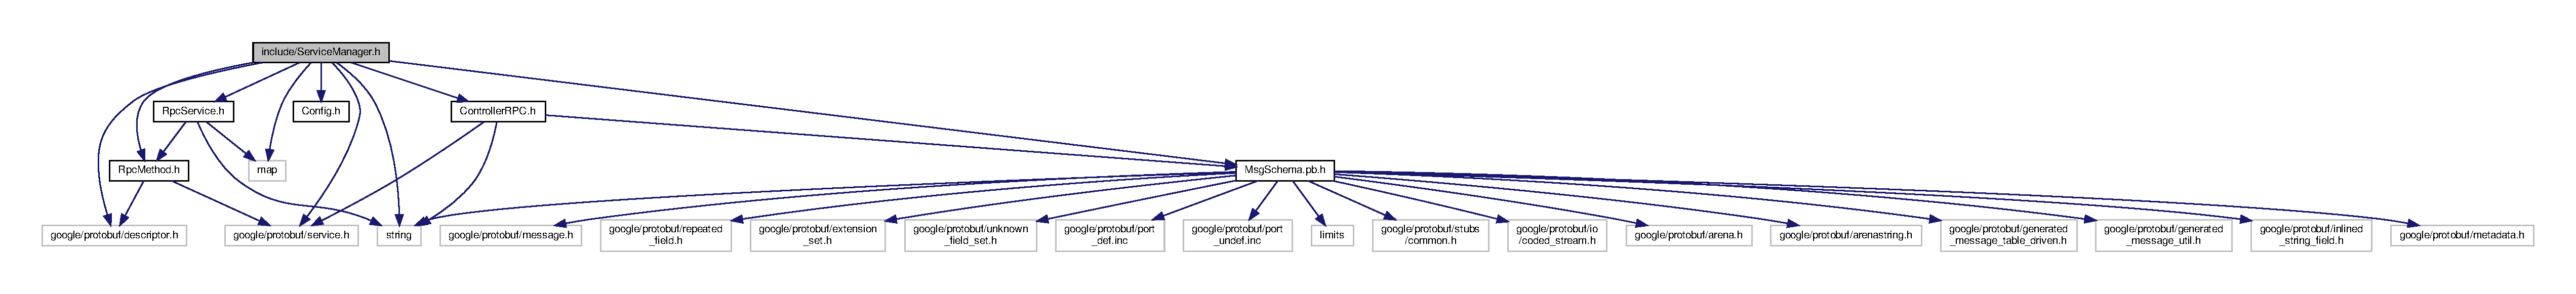
\includegraphics[width=350pt]{ServiceManager_8h__incl}
\end{center}
\end{figure}
This graph shows which files directly or indirectly include this file\+:\nopagebreak
\begin{figure}[H]
\begin{center}
\leavevmode
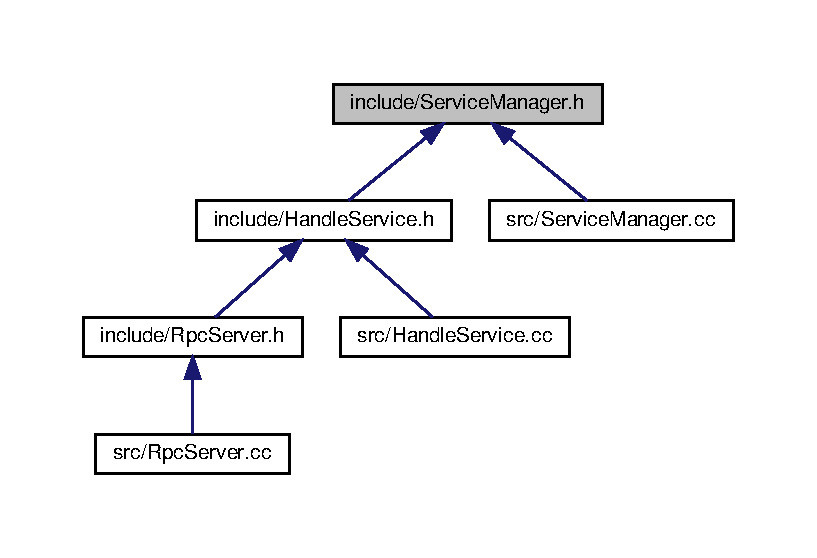
\includegraphics[width=350pt]{ServiceManager_8h__dep__incl}
\end{center}
\end{figure}
\subsection*{Classes}
\begin{DoxyCompactItemize}
\item 
class \hyperlink{classcoappbrpc_1_1ServiceManager}{coappbrpc\+::\+Service\+Manager}
\begin{DoxyCompactList}\small\item\em This class contains methods to handle R\+PC, register services, get services, get method details, validate passed parameters, validate requests, validate versions, and check if services are already existed or not. \end{DoxyCompactList}\end{DoxyCompactItemize}


\subsection{Detailed Description}
Handles Service creation, registration, getting and setting Services, handles R\+PC and validates requests. 


\chapter{Hierarchical Index}
\section{Class Hierarchy}
This inheritance list is sorted roughly, but not completely, alphabetically\+:\begin{DoxyCompactList}
\item \contentsline{section}{C}{\pageref{classC}}{}
\item \contentsline{section}{Client\+Params}{\pageref{structClientParams}}{}
\item \contentsline{section}{coappbrpc\+:\+:Coap\+Client}{\pageref{classcoappbrpc_1_1CoapClient}}{}
\item \contentsline{section}{Coap\+Common}{\pageref{classCoapCommon}}{}
\item Greeter\begin{DoxyCompactList}
\item \contentsline{section}{coappbrpc\+:\+:api\+:\+:Greeter\+Service\+Impl}{\pageref{classcoappbrpc_1_1api_1_1GreeterServiceImpl}}{}
\end{DoxyCompactList}
\item \contentsline{section}{Greeter\+Client}{\pageref{classGreeterClient}}{}
\item \contentsline{section}{Ping\+Client}{\pageref{classPingClient}}{}
\item Ping\+Service\begin{DoxyCompactList}
\item \contentsline{section}{coappbrpc\+:\+:api\+:\+:Ping\+Service\+Impl}{\pageref{classcoappbrpc_1_1api_1_1PingServiceImpl}}{}
\end{DoxyCompactList}
\item \contentsline{section}{coappbrpc\+:\+:Rpc\+Client}{\pageref{classcoappbrpc_1_1RpcClient}}{}
\item Rpc\+Controller\begin{DoxyCompactList}
\item \contentsline{section}{coappbrpc\+:\+:Controller\+R\+PC}{\pageref{classcoappbrpc_1_1ControllerRPC}}{}
\end{DoxyCompactList}
\item \contentsline{section}{coappbrpc\+:\+:Rpc\+Method}{\pageref{classcoappbrpc_1_1RpcMethod}}{}
\item \contentsline{section}{coappbrpc\+:\+:Rpc\+Server}{\pageref{classcoappbrpc_1_1RpcServer}}{}
\item \contentsline{section}{coappbrpc\+:\+:Rpc\+Service}{\pageref{classcoappbrpc_1_1RpcService}}{}
\item \contentsline{section}{coappbrpc\+:\+:Service\+Manager}{\pageref{classcoappbrpc_1_1ServiceManager}}{}
\end{DoxyCompactList}

\chapter{Class Index}
\section{Class List}
Here are the classes, structs, unions and interfaces with brief descriptions\+:\begin{DoxyCompactList}
\item\contentsline{section}{\hyperlink{structClientParams}{Client\+Params} }{\pageref{structClientParams}}{}
\item\contentsline{section}{\hyperlink{classcoappbrpc_1_1ClientRPC}{coappbrpc\+::\+Client\+R\+PC} }{\pageref{classcoappbrpc_1_1ClientRPC}}{}
\item\contentsline{section}{\hyperlink{classClientStub}{Client\+Stub} }{\pageref{classClientStub}}{}
\item\contentsline{section}{\hyperlink{classcoappbrpc_1_1CoapClient}{coappbrpc\+::\+Coap\+Client} }{\pageref{classcoappbrpc_1_1CoapClient}}{}
\item\contentsline{section}{\hyperlink{classCoapCommon}{Coap\+Common} }{\pageref{classCoapCommon}}{}
\item\contentsline{section}{\hyperlink{classcoappbrpc_1_1ControllerRPC}{coappbrpc\+::\+Controller\+R\+PC} }{\pageref{classcoappbrpc_1_1ControllerRPC}}{}
\item\contentsline{section}{\hyperlink{classcoappbrpc_1_1Error}{coappbrpc\+::\+Error} }{\pageref{classcoappbrpc_1_1Error}}{}
\item\contentsline{section}{\hyperlink{classcoappbrpc_1_1ErrorDefaultTypeInternal}{coappbrpc\+::\+Error\+Default\+Type\+Internal} }{\pageref{classcoappbrpc_1_1ErrorDefaultTypeInternal}}{}
\item\contentsline{section}{\hyperlink{classGreeterClient}{Greeter\+Client} }{\pageref{classGreeterClient}}{}
\item\contentsline{section}{\hyperlink{classcoappbrpc_1_1api_1_1GreeterServiceImpl}{coappbrpc\+::api\+::\+Greeter\+Service\+Impl} }{\pageref{classcoappbrpc_1_1api_1_1GreeterServiceImpl}}{}
\item\contentsline{section}{\hyperlink{classcoappbrpc_1_1api_1_1PingRequest_1_1HasBitSetters}{coappbrpc\+::api\+::\+Ping\+Request\+::\+Has\+Bit\+Setters} }{\pageref{classcoappbrpc_1_1api_1_1PingRequest_1_1HasBitSetters}}{}
\item\contentsline{section}{\hyperlink{classcoappbrpc_1_1Request_1_1HasBitSetters}{coappbrpc\+::\+Request\+::\+Has\+Bit\+Setters} }{\pageref{classcoappbrpc_1_1Request_1_1HasBitSetters}}{}
\item\contentsline{section}{\hyperlink{classcoappbrpc_1_1api_1_1PingResponse_1_1HasBitSetters}{coappbrpc\+::api\+::\+Ping\+Response\+::\+Has\+Bit\+Setters} }{\pageref{classcoappbrpc_1_1api_1_1PingResponse_1_1HasBitSetters}}{}
\item\contentsline{section}{\hyperlink{classcoappbrpc_1_1Error_1_1HasBitSetters}{coappbrpc\+::\+Error\+::\+Has\+Bit\+Setters} }{\pageref{classcoappbrpc_1_1Error_1_1HasBitSetters}}{}
\item\contentsline{section}{\hyperlink{classcoappbrpc_1_1Response_1_1HasBitSetters}{coappbrpc\+::\+Response\+::\+Has\+Bit\+Setters} }{\pageref{classcoappbrpc_1_1Response_1_1HasBitSetters}}{}
\item\contentsline{section}{\hyperlink{classcoappbrpc_1_1MethodRPC}{coappbrpc\+::\+Method\+R\+PC} }{\pageref{classcoappbrpc_1_1MethodRPC}}{}
\item\contentsline{section}{\hyperlink{classPingClient}{Ping\+Client} }{\pageref{classPingClient}}{}
\item\contentsline{section}{\hyperlink{classcoappbrpc_1_1api_1_1PingRequest}{coappbrpc\+::api\+::\+Ping\+Request} }{\pageref{classcoappbrpc_1_1api_1_1PingRequest}}{}
\item\contentsline{section}{\hyperlink{classcoappbrpc_1_1api_1_1PingRequestDefaultTypeInternal}{coappbrpc\+::api\+::\+Ping\+Request\+Default\+Type\+Internal} }{\pageref{classcoappbrpc_1_1api_1_1PingRequestDefaultTypeInternal}}{}
\item\contentsline{section}{\hyperlink{classcoappbrpc_1_1api_1_1PingResponse}{coappbrpc\+::api\+::\+Ping\+Response} }{\pageref{classcoappbrpc_1_1api_1_1PingResponse}}{}
\item\contentsline{section}{\hyperlink{classcoappbrpc_1_1api_1_1PingResponseDefaultTypeInternal}{coappbrpc\+::api\+::\+Ping\+Response\+Default\+Type\+Internal} }{\pageref{classcoappbrpc_1_1api_1_1PingResponseDefaultTypeInternal}}{}
\item\contentsline{section}{\hyperlink{classcoappbrpc_1_1api_1_1PingService}{coappbrpc\+::api\+::\+Ping\+Service} }{\pageref{classcoappbrpc_1_1api_1_1PingService}}{}
\item\contentsline{section}{\hyperlink{classcoappbrpc_1_1api_1_1PingService__Stub}{coappbrpc\+::api\+::\+Ping\+Service\+\_\+\+Stub} }{\pageref{classcoappbrpc_1_1api_1_1PingService__Stub}}{}
\item\contentsline{section}{\hyperlink{classcoappbrpc_1_1api_1_1PingServiceImpl}{coappbrpc\+::api\+::\+Ping\+Service\+Impl} }{\pageref{classcoappbrpc_1_1api_1_1PingServiceImpl}}{}
\item\contentsline{section}{\hyperlink{classcoappbrpc_1_1Request}{coappbrpc\+::\+Request} }{\pageref{classcoappbrpc_1_1Request}}{}
\item\contentsline{section}{\hyperlink{classcoappbrpc_1_1RequestDefaultTypeInternal}{coappbrpc\+::\+Request\+Default\+Type\+Internal} }{\pageref{classcoappbrpc_1_1RequestDefaultTypeInternal}}{}
\item\contentsline{section}{\hyperlink{classcoappbrpc_1_1Response}{coappbrpc\+::\+Response} }{\pageref{classcoappbrpc_1_1Response}}{}
\item\contentsline{section}{\hyperlink{classcoappbrpc_1_1ResponseDefaultTypeInternal}{coappbrpc\+::\+Response\+Default\+Type\+Internal} }{\pageref{classcoappbrpc_1_1ResponseDefaultTypeInternal}}{}
\item\contentsline{section}{\hyperlink{classcoappbrpc_1_1ServerRPC}{coappbrpc\+::\+Server\+R\+PC} }{\pageref{classcoappbrpc_1_1ServerRPC}}{}
\item\contentsline{section}{\hyperlink{classcoappbrpc_1_1ServiceManager}{coappbrpc\+::\+Service\+Manager} }{\pageref{classcoappbrpc_1_1ServiceManager}}{}
\item\contentsline{section}{\hyperlink{classcoappbrpc_1_1ServiceRPC}{coappbrpc\+::\+Service\+R\+PC} }{\pageref{classcoappbrpc_1_1ServiceRPC}}{}
\item\contentsline{section}{\hyperlink{structTableStruct__MsgSchema__2eproto}{Table\+Struct\+\_\+\+Msg\+Schema\+\_\+2eproto} }{\pageref{structTableStruct__MsgSchema__2eproto}}{}
\item\contentsline{section}{\hyperlink{structTableStruct__rpc__5fping__2eproto}{Table\+Struct\+\_\+rpc\+\_\+5fping\+\_\+2eproto} }{\pageref{structTableStruct__rpc__5fping__2eproto}}{}
\end{DoxyCompactList}

\chapter{Class Documentation}
\hypertarget{structClientParams}{}\section{Client\+Params Struct Reference}
\label{structClientParams}\index{Client\+Params@{Client\+Params}}
\subsection*{Public Attributes}
\begin{DoxyCompactItemize}
\item 
\mbox{\Hypertarget{structClientParams_a3277dd9bc0fa8283a7d3b82d53f3c16a}\label{structClientParams_a3277dd9bc0fa8283a7d3b82d53f3c16a}} 
string {\bfseries addr}
\item 
\mbox{\Hypertarget{structClientParams_ade2b9a6084d6b1989c3440fe2cd60fdb}\label{structClientParams_ade2b9a6084d6b1989c3440fe2cd60fdb}} 
string {\bfseries port}
\item 
\mbox{\Hypertarget{structClientParams_aa40f37f1eeb3ed6cff8a76e92a7e9bd1}\label{structClientParams_aa40f37f1eeb3ed6cff8a76e92a7e9bd1}} 
int {\bfseries method\+Type}
\item 
\mbox{\Hypertarget{structClientParams_a6af6f3817ebf9ed3f7d9378e6a23a59e}\label{structClientParams_a6af6f3817ebf9ed3f7d9378e6a23a59e}} 
string {\bfseries interface}
\item 
\mbox{\Hypertarget{structClientParams_aa16d76f3cbdfa5bfd4e54bcdb9a25737}\label{structClientParams_aa16d76f3cbdfa5bfd4e54bcdb9a25737}} 
string {\bfseries payload}
\end{DoxyCompactItemize}


The documentation for this struct was generated from the following file\+:\begin{DoxyCompactItemize}
\item 
include/Coap\+Client.\+h\end{DoxyCompactItemize}

\hypertarget{classcoappbrpc_1_1ClientRPC}{}\section{coappbrpc\+:\+:Client\+R\+PC Class Reference}
\label{classcoappbrpc_1_1ClientRPC}\index{coappbrpc\+::\+Client\+R\+PC@{coappbrpc\+::\+Client\+R\+PC}}
\subsection*{Public Member Functions}
\begin{DoxyCompactItemize}
\item 
\mbox{\Hypertarget{classcoappbrpc_1_1ClientRPC_a53bb77d304bc17ab754a75fccd3a6372}\label{classcoappbrpc_1_1ClientRPC_a53bb77d304bc17ab754a75fccd3a6372}} 
void {\bfseries run\+Client} ()
\item 
\mbox{\Hypertarget{classcoappbrpc_1_1ClientRPC_a6331d4e08a096a14941ab1af7bdb1893}\label{classcoappbrpc_1_1ClientRPC_a6331d4e08a096a14941ab1af7bdb1893}} 
void {\bfseries set\+Response} (string)
\item 
\mbox{\Hypertarget{classcoappbrpc_1_1ClientRPC_a2ff7435d4a5ab5c8bf146b623c53f6d7}\label{classcoappbrpc_1_1ClientRPC_a2ff7435d4a5ab5c8bf146b623c53f6d7}} 
string {\bfseries get\+Response} ()
\item 
\mbox{\Hypertarget{classcoappbrpc_1_1ClientRPC_a1a97bb79af368c7f867157dd89e2a2e0}\label{classcoappbrpc_1_1ClientRPC_a1a97bb79af368c7f867157dd89e2a2e0}} 
void {\bfseries set\+Server\+Addr} (string, string)
\item 
\mbox{\Hypertarget{classcoappbrpc_1_1ClientRPC_adb36f3777ba6ffba5a85a93acb3e6718}\label{classcoappbrpc_1_1ClientRPC_adb36f3777ba6ffba5a85a93acb3e6718}} 
\hyperlink{classcoappbrpc_1_1Response}{Response} {\bfseries exec\+Func} (string, string, string, string)
\end{DoxyCompactItemize}
\subsection*{Static Public Member Functions}
\begin{DoxyCompactItemize}
\item 
\mbox{\Hypertarget{classcoappbrpc_1_1ClientRPC_aaae393ce4bcf1200e631b0fe39f54f42}\label{classcoappbrpc_1_1ClientRPC_aaae393ce4bcf1200e631b0fe39f54f42}} 
static \hyperlink{classcoappbrpc_1_1ClientRPC}{Client\+R\+PC} $\ast$ {\bfseries get\+Instance} ()
\end{DoxyCompactItemize}


The documentation for this class was generated from the following files\+:\begin{DoxyCompactItemize}
\item 
include/Client\+R\+P\+C.\+h\item 
src/Client\+R\+P\+C.\+cc\end{DoxyCompactItemize}

\hypertarget{classClientStub}{}\section{Client\+Stub Class Reference}
\label{classClientStub}\index{Client\+Stub@{Client\+Stub}}
\subsection*{Public Member Functions}
\begin{DoxyCompactItemize}
\item 
\mbox{\Hypertarget{classClientStub_a423d4c727b14421503be1bc43780ee85}\label{classClientStub_a423d4c727b14421503be1bc43780ee85}} 
void {\bfseries Ping} (Ping\+Request, Ping\+Response $\ast$)
\end{DoxyCompactItemize}


The documentation for this class was generated from the following files\+:\begin{DoxyCompactItemize}
\item 
example/ping/Client\+Stub.\+h\item 
example/ping/Client\+Stub.\+cc\item 
generator/templates/Client\+Stub\+Template.\+cc\end{DoxyCompactItemize}

\hypertarget{classcoappbrpc_1_1CoapClient}{}\section{coappbrpc\+:\+:Coap\+Client Class Reference}
\label{classcoappbrpc_1_1CoapClient}\index{coappbrpc\+::\+Coap\+Client@{coappbrpc\+::\+Coap\+Client}}


This class contains two methods to client\+Handler and execute\+Client client Handler is a callback function which returns response back to R\+PC client excute\+Client handles coap client request. It creates a coap context, uses U\+DP as transport controller, registers, adds options and creates P\+DU and sends to server.  




{\ttfamily \#include $<$Coap\+Client.\+h$>$}

\subsection*{Static Public Member Functions}
\begin{DoxyCompactItemize}
\item 
static void \hyperlink{classcoappbrpc_1_1CoapClient_ab27b2485df1e7213425fe0f1b75110fa}{client\+Handler} (struct coap\+\_\+context\+\_\+t $\ast$, coap\+\_\+session\+\_\+t $\ast$, coap\+\_\+pdu\+\_\+t $\ast$, coap\+\_\+pdu\+\_\+t $\ast$, const coap\+\_\+tid\+\_\+t)
\begin{DoxyCompactList}\small\item\em Callback function that sets response data to be sent back to R\+PC client. \end{DoxyCompactList}\item 
static int \hyperlink{classcoappbrpc_1_1CoapClient_ac622e2dd087135defc27d8d4401a3119}{execute\+Client} (\hyperlink{structClientParams}{Client\+Params})
\begin{DoxyCompactList}\small\item\em Handles coap client request, creates context, P\+D\+Us, uses U\+DP transport protocol, registers and adds coap option and sends request to coap server. \end{DoxyCompactList}\end{DoxyCompactItemize}
\subsection*{Public Attributes}
\begin{DoxyCompactItemize}
\item 
string \hyperlink{classcoappbrpc_1_1CoapClient_ae6909f236ca1cd6b8b6343b7827ea004}{payload}
\end{DoxyCompactItemize}


\subsection{Detailed Description}
This class contains two methods to client\+Handler and execute\+Client client Handler is a callback function which returns response back to R\+PC client excute\+Client handles coap client request. It creates a coap context, uses U\+DP as transport controller, registers, adds options and creates P\+DU and sends to server. 

\subsection{Member Function Documentation}
\mbox{\Hypertarget{classcoappbrpc_1_1CoapClient_ab27b2485df1e7213425fe0f1b75110fa}\label{classcoappbrpc_1_1CoapClient_ab27b2485df1e7213425fe0f1b75110fa}} 
\index{coappbrpc\+::\+Coap\+Client@{coappbrpc\+::\+Coap\+Client}!client\+Handler@{client\+Handler}}
\index{client\+Handler@{client\+Handler}!coappbrpc\+::\+Coap\+Client@{coappbrpc\+::\+Coap\+Client}}
\subsubsection{\texorpdfstring{client\+Handler()}{clientHandler()}}
{\footnotesize\ttfamily void coappbrpc\+::\+Coap\+Client\+::client\+Handler (\begin{DoxyParamCaption}\item[{struct coap\+\_\+context\+\_\+t $\ast$}]{ctx,  }\item[{coap\+\_\+session\+\_\+t $\ast$}]{session,  }\item[{coap\+\_\+pdu\+\_\+t $\ast$}]{sent,  }\item[{coap\+\_\+pdu\+\_\+t $\ast$}]{received,  }\item[{const coap\+\_\+tid\+\_\+t}]{id }\end{DoxyParamCaption})\hspace{0.3cm}{\ttfamily [static]}}



Callback function that sets response data to be sent back to R\+PC client. 


\begin{DoxyParams}{Parameters}
{\em ctx} & Coap context variable reference of type struct coap\+\_\+context\+\_\+t. \\
\hline
{\em session} & Coap Session variable reference of type coap\+\_\+session\+\_\+t \\
\hline
{\em sent} & Co\+AP P\+DU sent to the server \\
\hline
{\em received} & Co\+AP P\+DU received back from server \\
\hline
{\em id} & Co\+AP transaction Id of type const coap\+\_\+tid\+\_\+t \\
\hline
\end{DoxyParams}
\mbox{\Hypertarget{classcoappbrpc_1_1CoapClient_ac622e2dd087135defc27d8d4401a3119}\label{classcoappbrpc_1_1CoapClient_ac622e2dd087135defc27d8d4401a3119}} 
\index{coappbrpc\+::\+Coap\+Client@{coappbrpc\+::\+Coap\+Client}!execute\+Client@{execute\+Client}}
\index{execute\+Client@{execute\+Client}!coappbrpc\+::\+Coap\+Client@{coappbrpc\+::\+Coap\+Client}}
\subsubsection{\texorpdfstring{execute\+Client()}{executeClient()}}
{\footnotesize\ttfamily int coappbrpc\+::\+Coap\+Client\+::execute\+Client (\begin{DoxyParamCaption}\item[{\hyperlink{structClientParams}{Client\+Params}}]{params }\end{DoxyParamCaption})\hspace{0.3cm}{\ttfamily [static]}}



Handles coap client request, creates context, P\+D\+Us, uses U\+DP transport protocol, registers and adds coap option and sends request to coap server. 


\begin{DoxyParams}{Parameters}
{\em params} & Parameters of struct type \hyperlink{structClientParams}{Client\+Params} that comprises of all values required to sent to server \\
\hline
\end{DoxyParams}


\subsection{Member Data Documentation}
\mbox{\Hypertarget{classcoappbrpc_1_1CoapClient_ae6909f236ca1cd6b8b6343b7827ea004}\label{classcoappbrpc_1_1CoapClient_ae6909f236ca1cd6b8b6343b7827ea004}} 
\index{coappbrpc\+::\+Coap\+Client@{coappbrpc\+::\+Coap\+Client}!payload@{payload}}
\index{payload@{payload}!coappbrpc\+::\+Coap\+Client@{coappbrpc\+::\+Coap\+Client}}
\subsubsection{\texorpdfstring{payload}{payload}}
{\footnotesize\ttfamily string coappbrpc\+::\+Coap\+Client\+::payload}

string to hold value of payload 

The documentation for this class was generated from the following files\+:\begin{DoxyCompactItemize}
\item 
include/\hyperlink{CoapClient_8h}{Coap\+Client.\+h}\item 
src/\hyperlink{CoapClient_8cc}{Coap\+Client.\+cc}\end{DoxyCompactItemize}

\hypertarget{classCoapCommon}{}\section{Coap\+Common Class Reference}
\label{classCoapCommon}\index{Coap\+Common@{Coap\+Common}}


This class contains a function named resolve\+Address. This file is used and shared by both client and server side to verify ip addresses.  




{\ttfamily \#include $<$Coap\+Common.\+h$>$}

\subsection*{Static Public Member Functions}
\begin{DoxyCompactItemize}
\item 
static int \hyperlink{classCoapCommon_a3a2b20fe477be1c328f3ad0bc98f28dd}{resolve\+Address} (const char $\ast$, const char $\ast$, coap\+\_\+address\+\_\+t $\ast$)
\begin{DoxyCompactList}\small\item\em Resolves I\+Pv4 and I\+Pv6 addresses and shows error messages in case of error. \end{DoxyCompactList}\end{DoxyCompactItemize}


\subsection{Detailed Description}
This class contains a function named resolve\+Address. This file is used and shared by both client and server side to verify ip addresses. 

\subsection{Member Function Documentation}
\mbox{\Hypertarget{classCoapCommon_a3a2b20fe477be1c328f3ad0bc98f28dd}\label{classCoapCommon_a3a2b20fe477be1c328f3ad0bc98f28dd}} 
\index{Coap\+Common@{Coap\+Common}!resolve\+Address@{resolve\+Address}}
\index{resolve\+Address@{resolve\+Address}!Coap\+Common@{Coap\+Common}}
\subsubsection{\texorpdfstring{resolve\+Address()}{resolveAddress()}}
{\footnotesize\ttfamily int Coap\+Common\+::resolve\+Address (\begin{DoxyParamCaption}\item[{const char $\ast$}]{host,  }\item[{const char $\ast$}]{service,  }\item[{coap\+\_\+address\+\_\+t $\ast$}]{dst }\end{DoxyParamCaption})\hspace{0.3cm}{\ttfamily [static]}}



Resolves I\+Pv4 and I\+Pv6 addresses and shows error messages in case of error. 


\begin{DoxyParams}{Parameters}
{\em host} & I\+Pv4 or I\+Pv6(global) address \\
\hline
{\em service} & Port number \\
\hline
{\em dst} & Reference of a address of type coap\+\_\+address\+\_\+t, to store the result after resolving address \\
\hline
\end{DoxyParams}


The documentation for this class was generated from the following files\+:\begin{DoxyCompactItemize}
\item 
include/\hyperlink{CoapCommon_8h}{Coap\+Common.\+h}\item 
src/\hyperlink{CoapCommon_8cc}{Coap\+Common.\+cc}\end{DoxyCompactItemize}

\hypertarget{classcoappbrpc_1_1ControllerRPC}{}\section{coappbrpc\+:\+:Controller\+R\+PC Class Reference}
\label{classcoappbrpc_1_1ControllerRPC}\index{coappbrpc\+::\+Controller\+R\+PC@{coappbrpc\+::\+Controller\+R\+PC}}


This class inherits properties from google protobuf Rpc\+Controller, it has methods for resetting, setting failed, get error object if there is any error in the R\+PC.  




{\ttfamily \#include $<$Controller\+R\+P\+C.\+h$>$}



Inheritance diagram for coappbrpc\+:\+:Controller\+R\+PC\+:\nopagebreak
\begin{figure}[H]
\begin{center}
\leavevmode
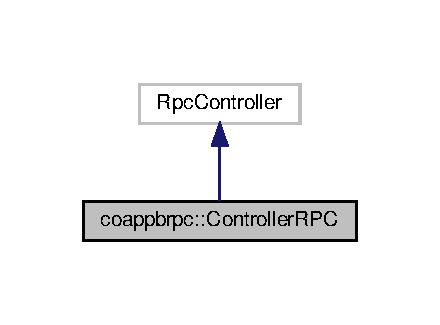
\includegraphics[width=211pt]{classcoappbrpc_1_1ControllerRPC__inherit__graph}
\end{center}
\end{figure}


Collaboration diagram for coappbrpc\+:\+:Controller\+R\+PC\+:\nopagebreak
\begin{figure}[H]
\begin{center}
\leavevmode
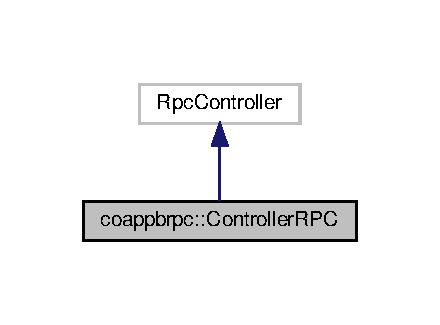
\includegraphics[width=211pt]{classcoappbrpc_1_1ControllerRPC__coll__graph}
\end{center}
\end{figure}
\subsection*{Public Member Functions}
\begin{DoxyCompactItemize}
\item 
\mbox{\Hypertarget{classcoappbrpc_1_1ControllerRPC_aac8d7a0e52a017d60a411a462bad6d91}\label{classcoappbrpc_1_1ControllerRPC_aac8d7a0e52a017d60a411a462bad6d91}} 
void \hyperlink{classcoappbrpc_1_1ControllerRPC_aac8d7a0e52a017d60a411a462bad6d91}{Reset} ()
\begin{DoxyCompactList}\small\item\em Resets m\+\_\+failed flag to false. \end{DoxyCompactList}\item 
\mbox{\Hypertarget{classcoappbrpc_1_1ControllerRPC_a20a3b119687bea2ac836db07a3b04287}\label{classcoappbrpc_1_1ControllerRPC_a20a3b119687bea2ac836db07a3b04287}} 
bool \hyperlink{classcoappbrpc_1_1ControllerRPC_a20a3b119687bea2ac836db07a3b04287}{Failed} () const
\begin{DoxyCompactList}\small\item\em getter function that returns m\+\_\+failed flag \end{DoxyCompactList}\item 
\mbox{\Hypertarget{classcoappbrpc_1_1ControllerRPC_a96035415234221d2972a3f2f790275ce}\label{classcoappbrpc_1_1ControllerRPC_a96035415234221d2972a3f2f790275ce}} 
string \hyperlink{classcoappbrpc_1_1ControllerRPC_a96035415234221d2972a3f2f790275ce}{Error\+Text} () const
\begin{DoxyCompactList}\small\item\em Getter function that returns message stored in m\+\_\+message. \end{DoxyCompactList}\item 
void \hyperlink{classcoappbrpc_1_1ControllerRPC_a3d91a6d0ba16232c531c3313e4412212}{Set\+Failed} (const string \&reason)
\begin{DoxyCompactList}\small\item\em Setter function which sets m\+\_\+failed to true when R\+PC fails and set m\+\_\+message to the reason of failure sent as parameter. \end{DoxyCompactList}\item 
void \hyperlink{classcoappbrpc_1_1ControllerRPC_a480586532b344e3ca8da2d2519ba593f}{append\+Failed} (const string \&reason)
\begin{DoxyCompactList}\small\item\em Function that appends multiple reasons for failure. \end{DoxyCompactList}\item 
\mbox{\Hypertarget{classcoappbrpc_1_1ControllerRPC_aab955bb22c799e5d544b3083fe64c7d7}\label{classcoappbrpc_1_1ControllerRPC_aab955bb22c799e5d544b3083fe64c7d7}} 
Error \hyperlink{classcoappbrpc_1_1ControllerRPC_aab955bb22c799e5d544b3083fe64c7d7}{error\+Obj} (void) const
\begin{DoxyCompactList}\small\item\em gets the Error object \end{DoxyCompactList}\item 
\mbox{\Hypertarget{classcoappbrpc_1_1ControllerRPC_a48a78ccc3c70a2135c78d612154e077c}\label{classcoappbrpc_1_1ControllerRPC_a48a78ccc3c70a2135c78d612154e077c}} 
void {\bfseries Start\+Cancel} ()
\item 
\mbox{\Hypertarget{classcoappbrpc_1_1ControllerRPC_ab6458ec248edf24fcc83b12a2573e13f}\label{classcoappbrpc_1_1ControllerRPC_ab6458ec248edf24fcc83b12a2573e13f}} 
bool {\bfseries Is\+Canceled} () const
\item 
\mbox{\Hypertarget{classcoappbrpc_1_1ControllerRPC_abc9385d7476171035cffb779c7966f89}\label{classcoappbrpc_1_1ControllerRPC_abc9385d7476171035cffb779c7966f89}} 
void {\bfseries Notify\+On\+Cancel} (Closure $\ast$callback)
\end{DoxyCompactItemize}


\subsection{Detailed Description}
This class inherits properties from google protobuf Rpc\+Controller, it has methods for resetting, setting failed, get error object if there is any error in the R\+PC. 

\subsection{Member Function Documentation}
\mbox{\Hypertarget{classcoappbrpc_1_1ControllerRPC_a480586532b344e3ca8da2d2519ba593f}\label{classcoappbrpc_1_1ControllerRPC_a480586532b344e3ca8da2d2519ba593f}} 
\index{coappbrpc\+::\+Controller\+R\+PC@{coappbrpc\+::\+Controller\+R\+PC}!append\+Failed@{append\+Failed}}
\index{append\+Failed@{append\+Failed}!coappbrpc\+::\+Controller\+R\+PC@{coappbrpc\+::\+Controller\+R\+PC}}
\subsubsection{\texorpdfstring{append\+Failed()}{appendFailed()}}
{\footnotesize\ttfamily void coappbrpc\+::\+Controller\+R\+P\+C\+::append\+Failed (\begin{DoxyParamCaption}\item[{const string \&}]{reason }\end{DoxyParamCaption})\hspace{0.3cm}{\ttfamily [inline]}}



Function that appends multiple reasons for failure. 


\begin{DoxyParams}{Parameters}
{\em reason} & string value that has explanation for failure \\
\hline
\end{DoxyParams}
\mbox{\Hypertarget{classcoappbrpc_1_1ControllerRPC_a3d91a6d0ba16232c531c3313e4412212}\label{classcoappbrpc_1_1ControllerRPC_a3d91a6d0ba16232c531c3313e4412212}} 
\index{coappbrpc\+::\+Controller\+R\+PC@{coappbrpc\+::\+Controller\+R\+PC}!Set\+Failed@{Set\+Failed}}
\index{Set\+Failed@{Set\+Failed}!coappbrpc\+::\+Controller\+R\+PC@{coappbrpc\+::\+Controller\+R\+PC}}
\subsubsection{\texorpdfstring{Set\+Failed()}{SetFailed()}}
{\footnotesize\ttfamily void coappbrpc\+::\+Controller\+R\+P\+C\+::\+Set\+Failed (\begin{DoxyParamCaption}\item[{const string \&}]{reason }\end{DoxyParamCaption})\hspace{0.3cm}{\ttfamily [inline]}}



Setter function which sets m\+\_\+failed to true when R\+PC fails and set m\+\_\+message to the reason of failure sent as parameter. 


\begin{DoxyParams}{Parameters}
{\em reason} & string value that has explanation for failure \\
\hline
\end{DoxyParams}


The documentation for this class was generated from the following file\+:\begin{DoxyCompactItemize}
\item 
include/\hyperlink{ControllerRPC_8h}{Controller\+R\+P\+C.\+h}\end{DoxyCompactItemize}

\hypertarget{classcoappbrpc_1_1Error}{}\section{coappbrpc\+:\+:Error Class Reference}
\label{classcoappbrpc_1_1Error}\index{coappbrpc\+::\+Error@{coappbrpc\+::\+Error}}


Inheritance diagram for coappbrpc\+:\+:Error\+:\nopagebreak
\begin{figure}[H]
\begin{center}
\leavevmode
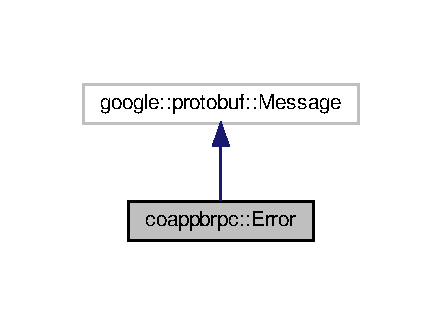
\includegraphics[width=212pt]{classcoappbrpc_1_1Error__inherit__graph}
\end{center}
\end{figure}


Collaboration diagram for coappbrpc\+:\+:Error\+:\nopagebreak
\begin{figure}[H]
\begin{center}
\leavevmode
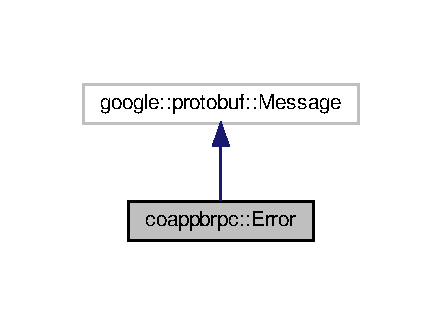
\includegraphics[width=212pt]{classcoappbrpc_1_1Error__coll__graph}
\end{center}
\end{figure}
\subsection*{Classes}
\begin{DoxyCompactItemize}
\item 
class \hyperlink{classcoappbrpc_1_1Error_1_1HasBitSetters}{Has\+Bit\+Setters}
\end{DoxyCompactItemize}
\subsection*{Public Member Functions}
\begin{DoxyCompactItemize}
\item 
\mbox{\Hypertarget{classcoappbrpc_1_1Error_a1a325665c85fc96f082a311cb3e3fc23}\label{classcoappbrpc_1_1Error_a1a325665c85fc96f082a311cb3e3fc23}} 
{\bfseries Error} (const \hyperlink{classcoappbrpc_1_1Error}{Error} \&from)
\item 
\mbox{\Hypertarget{classcoappbrpc_1_1Error_a06adcbeeca663447f9cf0387740f0744}\label{classcoappbrpc_1_1Error_a06adcbeeca663447f9cf0387740f0744}} 
\hyperlink{classcoappbrpc_1_1Error}{Error} \& {\bfseries operator=} (const \hyperlink{classcoappbrpc_1_1Error}{Error} \&from)
\item 
\mbox{\Hypertarget{classcoappbrpc_1_1Error_a0e09aab9715bdfa1c467f9ca7c4ed75a}\label{classcoappbrpc_1_1Error_a0e09aab9715bdfa1c467f9ca7c4ed75a}} 
void {\bfseries Swap} (\hyperlink{classcoappbrpc_1_1Error}{Error} $\ast$other)
\item 
\mbox{\Hypertarget{classcoappbrpc_1_1Error_ae52bf2329532524ec95a3e60225a62a2}\label{classcoappbrpc_1_1Error_ae52bf2329532524ec95a3e60225a62a2}} 
\hyperlink{classcoappbrpc_1_1Error}{Error} $\ast$ {\bfseries New} () const final
\item 
\mbox{\Hypertarget{classcoappbrpc_1_1Error_ac4bce964cb8730485d628a206af6d117}\label{classcoappbrpc_1_1Error_ac4bce964cb8730485d628a206af6d117}} 
\hyperlink{classcoappbrpc_1_1Error}{Error} $\ast$ {\bfseries New} (\+::google\+::protobuf\+::\+Arena $\ast$arena) const final
\item 
\mbox{\Hypertarget{classcoappbrpc_1_1Error_abf9ba3b9723a2d981aaf83d22ec8757a}\label{classcoappbrpc_1_1Error_abf9ba3b9723a2d981aaf83d22ec8757a}} 
void {\bfseries Copy\+From} (const \+::google\+::protobuf\+::\+Message \&from) final
\item 
\mbox{\Hypertarget{classcoappbrpc_1_1Error_ab853399916ca41d8eaa2aab0535533d0}\label{classcoappbrpc_1_1Error_ab853399916ca41d8eaa2aab0535533d0}} 
void {\bfseries Merge\+From} (const \+::google\+::protobuf\+::\+Message \&from) final
\item 
\mbox{\Hypertarget{classcoappbrpc_1_1Error_a52ca8b242a78f111be7735895160a1a3}\label{classcoappbrpc_1_1Error_a52ca8b242a78f111be7735895160a1a3}} 
void {\bfseries Copy\+From} (const \hyperlink{classcoappbrpc_1_1Error}{Error} \&from)
\item 
\mbox{\Hypertarget{classcoappbrpc_1_1Error_a9b8eca3a850aa4c53c8b46203c2dbffd}\label{classcoappbrpc_1_1Error_a9b8eca3a850aa4c53c8b46203c2dbffd}} 
void {\bfseries Merge\+From} (const \hyperlink{classcoappbrpc_1_1Error}{Error} \&from)
\item 
\mbox{\Hypertarget{classcoappbrpc_1_1Error_ad9e04e9f321d36f7f4fd97847cd228ce}\label{classcoappbrpc_1_1Error_ad9e04e9f321d36f7f4fd97847cd228ce}} 
void {\bfseries Clear} () final
\item 
\mbox{\Hypertarget{classcoappbrpc_1_1Error_ad9724721599eacc6eede185afac48793}\label{classcoappbrpc_1_1Error_ad9724721599eacc6eede185afac48793}} 
bool {\bfseries Is\+Initialized} () const final
\item 
\mbox{\Hypertarget{classcoappbrpc_1_1Error_aa858f0fd915c5692b4de0b551cb93b81}\label{classcoappbrpc_1_1Error_aa858f0fd915c5692b4de0b551cb93b81}} 
size\+\_\+t {\bfseries Byte\+Size\+Long} () const final
\item 
\mbox{\Hypertarget{classcoappbrpc_1_1Error_a615a3c932e6c7c1756cd1e53438cb119}\label{classcoappbrpc_1_1Error_a615a3c932e6c7c1756cd1e53438cb119}} 
bool {\bfseries Merge\+Partial\+From\+Coded\+Stream} (\+::google\+::protobuf\+::io\+::\+Coded\+Input\+Stream $\ast$input) final
\item 
\mbox{\Hypertarget{classcoappbrpc_1_1Error_a5cda1b9ed16feec0777bcbcf76f89c1e}\label{classcoappbrpc_1_1Error_a5cda1b9ed16feec0777bcbcf76f89c1e}} 
void {\bfseries Serialize\+With\+Cached\+Sizes} (\+::google\+::protobuf\+::io\+::\+Coded\+Output\+Stream $\ast$output) const final
\item 
\mbox{\Hypertarget{classcoappbrpc_1_1Error_a30aa6e3b7dbd72eabb6e1d962de68e8d}\label{classcoappbrpc_1_1Error_a30aa6e3b7dbd72eabb6e1d962de68e8d}} 
\+::google\+::protobuf\+::uint8 $\ast$ {\bfseries Internal\+Serialize\+With\+Cached\+Sizes\+To\+Array} (bool deterministic, \+::google\+::protobuf\+::uint8 $\ast$target) const final
\item 
\mbox{\Hypertarget{classcoappbrpc_1_1Error_a9b79b7d43fbbbb4f2e9172a1f898aeb4}\label{classcoappbrpc_1_1Error_a9b79b7d43fbbbb4f2e9172a1f898aeb4}} 
int {\bfseries Get\+Cached\+Size} () const final
\item 
\mbox{\Hypertarget{classcoappbrpc_1_1Error_a8803f21e0ec88ebc884b39923cfd3c7f}\label{classcoappbrpc_1_1Error_a8803f21e0ec88ebc884b39923cfd3c7f}} 
\+::google\+::protobuf\+::\+Metadata {\bfseries Get\+Metadata} () const final
\item 
\mbox{\Hypertarget{classcoappbrpc_1_1Error_a577934032656de1fa052835cad23626a}\label{classcoappbrpc_1_1Error_a577934032656de1fa052835cad23626a}} 
void {\bfseries clear\+\_\+message} ()
\item 
\mbox{\Hypertarget{classcoappbrpc_1_1Error_a9dc400abcdf851cec58bc02ebd2392cc}\label{classcoappbrpc_1_1Error_a9dc400abcdf851cec58bc02ebd2392cc}} 
const \+::std\+::string \& {\bfseries message} () const
\item 
\mbox{\Hypertarget{classcoappbrpc_1_1Error_a11354fca41ecfb10b1ae201c6232c8fd}\label{classcoappbrpc_1_1Error_a11354fca41ecfb10b1ae201c6232c8fd}} 
void {\bfseries set\+\_\+message} (const \+::std\+::string \&value)
\item 
\mbox{\Hypertarget{classcoappbrpc_1_1Error_ac7f5e9392eb8c448e87f23903c19c8aa}\label{classcoappbrpc_1_1Error_ac7f5e9392eb8c448e87f23903c19c8aa}} 
void {\bfseries set\+\_\+message} (const char $\ast$value)
\item 
\mbox{\Hypertarget{classcoappbrpc_1_1Error_a62ff01b3ac63dab5cb5b0f9c6973a5de}\label{classcoappbrpc_1_1Error_a62ff01b3ac63dab5cb5b0f9c6973a5de}} 
void {\bfseries set\+\_\+message} (const char $\ast$value, size\+\_\+t size)
\item 
\mbox{\Hypertarget{classcoappbrpc_1_1Error_a8b7ad03301f0e7ac9651f01144dbf82a}\label{classcoappbrpc_1_1Error_a8b7ad03301f0e7ac9651f01144dbf82a}} 
\+::std\+::string $\ast$ {\bfseries mutable\+\_\+message} ()
\item 
\mbox{\Hypertarget{classcoappbrpc_1_1Error_ab69f3ef2b76905f9843e9871c11a2d90}\label{classcoappbrpc_1_1Error_ab69f3ef2b76905f9843e9871c11a2d90}} 
\+::std\+::string $\ast$ {\bfseries release\+\_\+message} ()
\item 
\mbox{\Hypertarget{classcoappbrpc_1_1Error_aa481822f68e60ecd862635c6f2e3e397}\label{classcoappbrpc_1_1Error_aa481822f68e60ecd862635c6f2e3e397}} 
void {\bfseries set\+\_\+allocated\+\_\+message} (\+::std\+::string $\ast$message)
\item 
\mbox{\Hypertarget{classcoappbrpc_1_1Error_a223825c785dffa0c6184dba20c474a86}\label{classcoappbrpc_1_1Error_a223825c785dffa0c6184dba20c474a86}} 
void {\bfseries clear\+\_\+data} ()
\item 
\mbox{\Hypertarget{classcoappbrpc_1_1Error_af9cfa2e6266aeb1294ffef65da39da96}\label{classcoappbrpc_1_1Error_af9cfa2e6266aeb1294ffef65da39da96}} 
const \+::std\+::string \& {\bfseries data} () const
\item 
\mbox{\Hypertarget{classcoappbrpc_1_1Error_a1e65c8c348e8852ef6846621b317f22a}\label{classcoappbrpc_1_1Error_a1e65c8c348e8852ef6846621b317f22a}} 
void {\bfseries set\+\_\+data} (const \+::std\+::string \&value)
\item 
\mbox{\Hypertarget{classcoappbrpc_1_1Error_a71c4fff56dc64991d4b3aecf24778ad2}\label{classcoappbrpc_1_1Error_a71c4fff56dc64991d4b3aecf24778ad2}} 
void {\bfseries set\+\_\+data} (const char $\ast$value)
\item 
\mbox{\Hypertarget{classcoappbrpc_1_1Error_ab6fce8187d7f8b32aa627c394ff21ce1}\label{classcoappbrpc_1_1Error_ab6fce8187d7f8b32aa627c394ff21ce1}} 
void {\bfseries set\+\_\+data} (const void $\ast$value, size\+\_\+t size)
\item 
\mbox{\Hypertarget{classcoappbrpc_1_1Error_a43f80373d6775e1863b355c0bd80ac18}\label{classcoappbrpc_1_1Error_a43f80373d6775e1863b355c0bd80ac18}} 
\+::std\+::string $\ast$ {\bfseries mutable\+\_\+data} ()
\item 
\mbox{\Hypertarget{classcoappbrpc_1_1Error_ae54fc2d7f0a102d5b7a3b55a61bd96a1}\label{classcoappbrpc_1_1Error_ae54fc2d7f0a102d5b7a3b55a61bd96a1}} 
\+::std\+::string $\ast$ {\bfseries release\+\_\+data} ()
\item 
\mbox{\Hypertarget{classcoappbrpc_1_1Error_aeae3dd27dabf24258646616365846a22}\label{classcoappbrpc_1_1Error_aeae3dd27dabf24258646616365846a22}} 
void {\bfseries set\+\_\+allocated\+\_\+data} (\+::std\+::string $\ast$data)
\end{DoxyCompactItemize}
\subsection*{Static Public Member Functions}
\begin{DoxyCompactItemize}
\item 
\mbox{\Hypertarget{classcoappbrpc_1_1Error_a835816ae390a4823c3cda44d0eea4ac2}\label{classcoappbrpc_1_1Error_a835816ae390a4823c3cda44d0eea4ac2}} 
static const \+::google\+::protobuf\+::\+Descriptor $\ast$ {\bfseries descriptor} ()
\item 
\mbox{\Hypertarget{classcoappbrpc_1_1Error_ae4e0a093db086c07b372c9fed1b76b18}\label{classcoappbrpc_1_1Error_ae4e0a093db086c07b372c9fed1b76b18}} 
static const \hyperlink{classcoappbrpc_1_1Error}{Error} \& {\bfseries default\+\_\+instance} ()
\item 
\mbox{\Hypertarget{classcoappbrpc_1_1Error_a9ef5aed94b431be32ae561055e86da91}\label{classcoappbrpc_1_1Error_a9ef5aed94b431be32ae561055e86da91}} 
static void {\bfseries Init\+As\+Default\+Instance} ()
\item 
\mbox{\Hypertarget{classcoappbrpc_1_1Error_a054f12c7ba5aa48ac9e29c89eadfa00f}\label{classcoappbrpc_1_1Error_a054f12c7ba5aa48ac9e29c89eadfa00f}} 
static const \hyperlink{classcoappbrpc_1_1Error}{Error} $\ast$ {\bfseries internal\+\_\+default\+\_\+instance} ()
\end{DoxyCompactItemize}
\subsection*{Static Public Attributes}
\begin{DoxyCompactItemize}
\item 
static constexpr int {\bfseries k\+Index\+In\+File\+Messages}
\item 
\mbox{\Hypertarget{classcoappbrpc_1_1Error_ac3b04639b8436127975805d710defdaa}\label{classcoappbrpc_1_1Error_ac3b04639b8436127975805d710defdaa}} 
static const int {\bfseries k\+Message\+Field\+Number} = 1
\item 
\mbox{\Hypertarget{classcoappbrpc_1_1Error_afdf01e84439d824f3f8276b0fc18189a}\label{classcoappbrpc_1_1Error_afdf01e84439d824f3f8276b0fc18189a}} 
static const int {\bfseries k\+Data\+Field\+Number} = 2
\end{DoxyCompactItemize}
\subsection*{Friends}
\begin{DoxyCompactItemize}
\item 
\mbox{\Hypertarget{classcoappbrpc_1_1Error_a65c087bf06ded9c9be363691f7b7bafa}\label{classcoappbrpc_1_1Error_a65c087bf06ded9c9be363691f7b7bafa}} 
struct {\bfseries \+::\+Table\+Struct\+\_\+\+Msg\+Schema\+\_\+2eproto}
\item 
\mbox{\Hypertarget{classcoappbrpc_1_1Error_a8a56a72c6855aff317cf18b3c5f2fa5d}\label{classcoappbrpc_1_1Error_a8a56a72c6855aff317cf18b3c5f2fa5d}} 
void {\bfseries swap} (\hyperlink{classcoappbrpc_1_1Error}{Error} \&a, \hyperlink{classcoappbrpc_1_1Error}{Error} \&b)
\end{DoxyCompactItemize}


\subsection{Member Data Documentation}
\mbox{\Hypertarget{classcoappbrpc_1_1Error_a92d90802862d90205267fb130aa544b9}\label{classcoappbrpc_1_1Error_a92d90802862d90205267fb130aa544b9}} 
\index{coappbrpc\+::\+Error@{coappbrpc\+::\+Error}!k\+Index\+In\+File\+Messages@{k\+Index\+In\+File\+Messages}}
\index{k\+Index\+In\+File\+Messages@{k\+Index\+In\+File\+Messages}!coappbrpc\+::\+Error@{coappbrpc\+::\+Error}}
\subsubsection{\texorpdfstring{k\+Index\+In\+File\+Messages}{kIndexInFileMessages}}
{\footnotesize\ttfamily constexpr int coappbrpc\+::\+Error\+::k\+Index\+In\+File\+Messages\hspace{0.3cm}{\ttfamily [static]}}

{\bfseries Initial value\+:}
\begin{DoxyCode}
=
    1
\end{DoxyCode}


The documentation for this class was generated from the following files\+:\begin{DoxyCompactItemize}
\item 
build/proto/Msg\+Schema.\+pb.\+h\item 
build/proto/Msg\+Schema.\+pb.\+cc\end{DoxyCompactItemize}

\hypertarget{classcoappbrpc_1_1ErrorDefaultTypeInternal}{}\section{coappbrpc\+:\+:Error\+Default\+Type\+Internal Class Reference}
\label{classcoappbrpc_1_1ErrorDefaultTypeInternal}\index{coappbrpc\+::\+Error\+Default\+Type\+Internal@{coappbrpc\+::\+Error\+Default\+Type\+Internal}}
\subsection*{Public Attributes}
\begin{DoxyCompactItemize}
\item 
\mbox{\Hypertarget{classcoappbrpc_1_1ErrorDefaultTypeInternal_ade1a1ad28e83164588942a5e28bf23c5}\label{classcoappbrpc_1_1ErrorDefaultTypeInternal_ade1a1ad28e83164588942a5e28bf23c5}} 
\+::google\+::protobuf\+::internal\+::\+Explicitly\+Constructed$<$ \hyperlink{classcoappbrpc_1_1Error}{Error} $>$ {\bfseries \+\_\+instance}
\end{DoxyCompactItemize}


The documentation for this class was generated from the following file\+:\begin{DoxyCompactItemize}
\item 
build/proto/Msg\+Schema.\+pb.\+cc\end{DoxyCompactItemize}

\hypertarget{classGreeterClient}{}\section{Greeter\+Client Class Reference}
\label{classGreeterClient}\index{Greeter\+Client@{Greeter\+Client}}
\subsection*{Public Member Functions}
\begin{DoxyCompactItemize}
\item 
\mbox{\Hypertarget{classGreeterClient_a673a567cdce22eeed0afaf48bf808fa8}\label{classGreeterClient_a673a567cdce22eeed0afaf48bf808fa8}} 
string {\bfseries Say\+Hello} (const std\+::string \&user)
\end{DoxyCompactItemize}


The documentation for this class was generated from the following file\+:\begin{DoxyCompactItemize}
\item 
example/helloworld/client.\+cpp\end{DoxyCompactItemize}

\hypertarget{classcoappbrpc_1_1api_1_1GreeterServiceImpl}{}\section{coappbrpc\+:\+:api\+:\+:Greeter\+Service\+Impl Class Reference}
\label{classcoappbrpc_1_1api_1_1GreeterServiceImpl}\index{coappbrpc\+::api\+::\+Greeter\+Service\+Impl@{coappbrpc\+::api\+::\+Greeter\+Service\+Impl}}


Inheritance diagram for coappbrpc\+:\+:api\+:\+:Greeter\+Service\+Impl\+:
\nopagebreak
\begin{figure}[H]
\begin{center}
\leavevmode
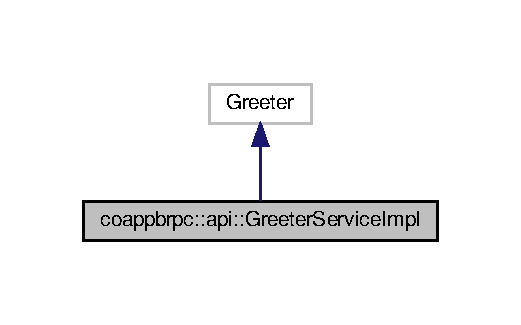
\includegraphics[width=250pt]{classcoappbrpc_1_1api_1_1GreeterServiceImpl__inherit__graph}
\end{center}
\end{figure}


Collaboration diagram for coappbrpc\+:\+:api\+:\+:Greeter\+Service\+Impl\+:
\nopagebreak
\begin{figure}[H]
\begin{center}
\leavevmode
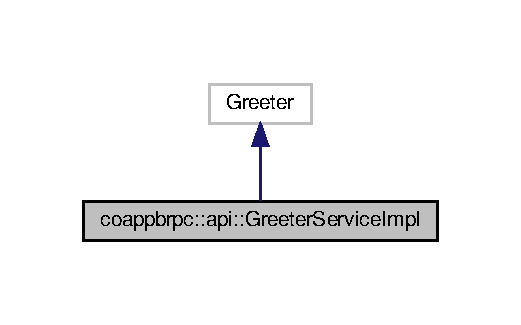
\includegraphics[width=250pt]{classcoappbrpc_1_1api_1_1GreeterServiceImpl__coll__graph}
\end{center}
\end{figure}
\subsection*{Public Member Functions}
\begin{DoxyCompactItemize}
\item 
\mbox{\Hypertarget{classcoappbrpc_1_1api_1_1GreeterServiceImpl_a009b97643d9728170104e367b8f40167}\label{classcoappbrpc_1_1api_1_1GreeterServiceImpl_a009b97643d9728170104e367b8f40167}} 
virtual void {\bfseries Say\+Hello} (Rpc\+Controller $\ast$controller, const Hello\+Request $\ast$request, Hello\+Reply $\ast$reply, Closure $\ast$done)
\end{DoxyCompactItemize}


The documentation for this class was generated from the following file\+:\begin{DoxyCompactItemize}
\item 
example/helloworld/server.\+cpp\end{DoxyCompactItemize}

\hypertarget{classcoappbrpc_1_1api_1_1PingRequest_1_1HasBitSetters}{}\section{coappbrpc\+:\+:api\+:\+:Ping\+Request\+:\+:Has\+Bit\+Setters Class Reference}
\label{classcoappbrpc_1_1api_1_1PingRequest_1_1HasBitSetters}\index{coappbrpc\+::api\+::\+Ping\+Request\+::\+Has\+Bit\+Setters@{coappbrpc\+::api\+::\+Ping\+Request\+::\+Has\+Bit\+Setters}}


The documentation for this class was generated from the following file\+:\begin{DoxyCompactItemize}
\item 
example/ping/rpc\+\_\+ping.\+pb.\+cc\end{DoxyCompactItemize}

\hypertarget{classcoappbrpc_1_1Request_1_1HasBitSetters}{}\section{coappbrpc\+:\+:Request\+:\+:Has\+Bit\+Setters Class Reference}
\label{classcoappbrpc_1_1Request_1_1HasBitSetters}\index{coappbrpc\+::\+Request\+::\+Has\+Bit\+Setters@{coappbrpc\+::\+Request\+::\+Has\+Bit\+Setters}}


The documentation for this class was generated from the following file\+:\begin{DoxyCompactItemize}
\item 
build/proto/Msg\+Schema.\+pb.\+cc\end{DoxyCompactItemize}

\hypertarget{classcoappbrpc_1_1api_1_1PingResponse_1_1HasBitSetters}{}\section{coappbrpc\+:\+:api\+:\+:Ping\+Response\+:\+:Has\+Bit\+Setters Class Reference}
\label{classcoappbrpc_1_1api_1_1PingResponse_1_1HasBitSetters}\index{coappbrpc\+::api\+::\+Ping\+Response\+::\+Has\+Bit\+Setters@{coappbrpc\+::api\+::\+Ping\+Response\+::\+Has\+Bit\+Setters}}


The documentation for this class was generated from the following file\+:\begin{DoxyCompactItemize}
\item 
example/ping/rpc\+\_\+ping.\+pb.\+cc\end{DoxyCompactItemize}

\hypertarget{classcoappbrpc_1_1Error_1_1HasBitSetters}{}\section{coappbrpc\+:\+:Error\+:\+:Has\+Bit\+Setters Class Reference}
\label{classcoappbrpc_1_1Error_1_1HasBitSetters}\index{coappbrpc\+::\+Error\+::\+Has\+Bit\+Setters@{coappbrpc\+::\+Error\+::\+Has\+Bit\+Setters}}


The documentation for this class was generated from the following file\+:\begin{DoxyCompactItemize}
\item 
build/proto/Msg\+Schema.\+pb.\+cc\end{DoxyCompactItemize}

\hypertarget{classcoappbrpc_1_1Response_1_1HasBitSetters}{}\section{coappbrpc\+:\+:Response\+:\+:Has\+Bit\+Setters Class Reference}
\label{classcoappbrpc_1_1Response_1_1HasBitSetters}\index{coappbrpc\+::\+Response\+::\+Has\+Bit\+Setters@{coappbrpc\+::\+Response\+::\+Has\+Bit\+Setters}}
\subsection*{Static Public Member Functions}
\begin{DoxyCompactItemize}
\item 
\mbox{\Hypertarget{classcoappbrpc_1_1Response_1_1HasBitSetters_afe7b2e5cad486fab4e12b8f92d20a5af}\label{classcoappbrpc_1_1Response_1_1HasBitSetters_afe7b2e5cad486fab4e12b8f92d20a5af}} 
static const \+::\hyperlink{classcoappbrpc_1_1Error}{coappbrpc\+::\+Error} \& {\bfseries error} (const \hyperlink{classcoappbrpc_1_1Response}{Response} $\ast$msg)
\end{DoxyCompactItemize}


The documentation for this class was generated from the following file\+:\begin{DoxyCompactItemize}
\item 
build/proto/Msg\+Schema.\+pb.\+cc\end{DoxyCompactItemize}

\hypertarget{classcoappbrpc_1_1MethodRPC}{}\section{coappbrpc\+:\+:Method\+R\+PC Class Reference}
\label{classcoappbrpc_1_1MethodRPC}\index{coappbrpc\+::\+Method\+R\+PC@{coappbrpc\+::\+Method\+R\+PC}}
\subsection*{Public Member Functions}
\begin{DoxyCompactItemize}
\item 
\mbox{\Hypertarget{classcoappbrpc_1_1MethodRPC_a0db09113d43fcfef728b4dd261cd564a}\label{classcoappbrpc_1_1MethodRPC_a0db09113d43fcfef728b4dd261cd564a}} 
{\bfseries Method\+R\+PC} (const Method\+Descriptor $\ast$\hyperlink{classcoappbrpc_1_1MethodRPC_a7e835872e8ec2768c3c4a8af2ddc9554}{descriptor}, const Message $\ast$\hyperlink{classcoappbrpc_1_1MethodRPC_abc03c65fd8f6a540dacc0a1a7cf64695}{request}, const Message $\ast$\hyperlink{classcoappbrpc_1_1MethodRPC_abf2e75cc873ba1b4591b78f9e1955d49}{response})
\end{DoxyCompactItemize}
\subsection*{Public Attributes}
\begin{DoxyCompactItemize}
\item 
const Method\+Descriptor $\ast$ \hyperlink{classcoappbrpc_1_1MethodRPC_a7e835872e8ec2768c3c4a8af2ddc9554}{descriptor}
\item 
const Message $\ast$ \hyperlink{classcoappbrpc_1_1MethodRPC_abc03c65fd8f6a540dacc0a1a7cf64695}{request}
\item 
const Message $\ast$ \hyperlink{classcoappbrpc_1_1MethodRPC_abf2e75cc873ba1b4591b78f9e1955d49}{response}
\end{DoxyCompactItemize}


\subsection{Member Data Documentation}
\mbox{\Hypertarget{classcoappbrpc_1_1MethodRPC_a7e835872e8ec2768c3c4a8af2ddc9554}\label{classcoappbrpc_1_1MethodRPC_a7e835872e8ec2768c3c4a8af2ddc9554}} 
\index{coappbrpc\+::\+Method\+R\+PC@{coappbrpc\+::\+Method\+R\+PC}!descriptor@{descriptor}}
\index{descriptor@{descriptor}!coappbrpc\+::\+Method\+R\+PC@{coappbrpc\+::\+Method\+R\+PC}}
\subsubsection{\texorpdfstring{descriptor}{descriptor}}
{\footnotesize\ttfamily const Method\+Descriptor$\ast$ coappbrpc\+::\+Method\+R\+P\+C\+::descriptor}

method descriptor \mbox{\Hypertarget{classcoappbrpc_1_1MethodRPC_abc03c65fd8f6a540dacc0a1a7cf64695}\label{classcoappbrpc_1_1MethodRPC_abc03c65fd8f6a540dacc0a1a7cf64695}} 
\index{coappbrpc\+::\+Method\+R\+PC@{coappbrpc\+::\+Method\+R\+PC}!request@{request}}
\index{request@{request}!coappbrpc\+::\+Method\+R\+PC@{coappbrpc\+::\+Method\+R\+PC}}
\subsubsection{\texorpdfstring{request}{request}}
{\footnotesize\ttfamily const Message$\ast$ coappbrpc\+::\+Method\+R\+P\+C\+::request}

parameters \mbox{\Hypertarget{classcoappbrpc_1_1MethodRPC_abf2e75cc873ba1b4591b78f9e1955d49}\label{classcoappbrpc_1_1MethodRPC_abf2e75cc873ba1b4591b78f9e1955d49}} 
\index{coappbrpc\+::\+Method\+R\+PC@{coappbrpc\+::\+Method\+R\+PC}!response@{response}}
\index{response@{response}!coappbrpc\+::\+Method\+R\+PC@{coappbrpc\+::\+Method\+R\+PC}}
\subsubsection{\texorpdfstring{response}{response}}
{\footnotesize\ttfamily const Message$\ast$ coappbrpc\+::\+Method\+R\+P\+C\+::response}

result 

The documentation for this class was generated from the following file\+:\begin{DoxyCompactItemize}
\item 
include/Method\+R\+P\+C.\+h\end{DoxyCompactItemize}

\hypertarget{classPingClient}{}\section{Ping\+Client Class Reference}
\label{classPingClient}\index{Ping\+Client@{Ping\+Client}}
\subsection*{Public Member Functions}
\begin{DoxyCompactItemize}
\item 
\mbox{\Hypertarget{classPingClient_a888873d874335defed11102c757e0612}\label{classPingClient_a888873d874335defed11102c757e0612}} 
string {\bfseries ping} (const string \&msg)
\end{DoxyCompactItemize}


The documentation for this class was generated from the following file\+:\begin{DoxyCompactItemize}
\item 
example/ping/client.\+cpp\end{DoxyCompactItemize}

\hypertarget{classcoappbrpc_1_1api_1_1PingRequest}{}\section{coappbrpc\+:\+:api\+:\+:Ping\+Request Class Reference}
\label{classcoappbrpc_1_1api_1_1PingRequest}\index{coappbrpc\+::api\+::\+Ping\+Request@{coappbrpc\+::api\+::\+Ping\+Request}}


Inheritance diagram for coappbrpc\+:\+:api\+:\+:Ping\+Request\+:
% FIG 0


Collaboration diagram for coappbrpc\+:\+:api\+:\+:Ping\+Request\+:
% FIG 1
\subsection*{Classes}
\begin{DoxyCompactItemize}
\item 
class \hyperlink{classcoappbrpc_1_1api_1_1PingRequest_1_1HasBitSetters}{Has\+Bit\+Setters}
\end{DoxyCompactItemize}
\subsection*{Public Member Functions}
\begin{DoxyCompactItemize}
\item 
\mbox{\Hypertarget{classcoappbrpc_1_1api_1_1PingRequest_a30f3255dfa8fc0e5135490461c1af728}\label{classcoappbrpc_1_1api_1_1PingRequest_a30f3255dfa8fc0e5135490461c1af728}} 
{\bfseries Ping\+Request} (const \hyperlink{classcoappbrpc_1_1api_1_1PingRequest}{Ping\+Request} \&from)
\item 
\mbox{\Hypertarget{classcoappbrpc_1_1api_1_1PingRequest_a9fea8caedf2419a70210aa1953526cd1}\label{classcoappbrpc_1_1api_1_1PingRequest_a9fea8caedf2419a70210aa1953526cd1}} 
\hyperlink{classcoappbrpc_1_1api_1_1PingRequest}{Ping\+Request} \& {\bfseries operator=} (const \hyperlink{classcoappbrpc_1_1api_1_1PingRequest}{Ping\+Request} \&from)
\item 
\mbox{\Hypertarget{classcoappbrpc_1_1api_1_1PingRequest_af756d05276d74ff2c3b324b1e0b38940}\label{classcoappbrpc_1_1api_1_1PingRequest_af756d05276d74ff2c3b324b1e0b38940}} 
void {\bfseries Swap} (\hyperlink{classcoappbrpc_1_1api_1_1PingRequest}{Ping\+Request} $\ast$other)
\item 
\mbox{\Hypertarget{classcoappbrpc_1_1api_1_1PingRequest_a871778bc2661c885172a53ef56819d86}\label{classcoappbrpc_1_1api_1_1PingRequest_a871778bc2661c885172a53ef56819d86}} 
\hyperlink{classcoappbrpc_1_1api_1_1PingRequest}{Ping\+Request} $\ast$ {\bfseries New} () const final
\item 
\mbox{\Hypertarget{classcoappbrpc_1_1api_1_1PingRequest_a24ecee4aa9edb3d40aae8fc2a13a4322}\label{classcoappbrpc_1_1api_1_1PingRequest_a24ecee4aa9edb3d40aae8fc2a13a4322}} 
\hyperlink{classcoappbrpc_1_1api_1_1PingRequest}{Ping\+Request} $\ast$ {\bfseries New} (\+::google\+::protobuf\+::\+Arena $\ast$arena) const final
\item 
\mbox{\Hypertarget{classcoappbrpc_1_1api_1_1PingRequest_a63f8978e82082a628f58dda8fce6331a}\label{classcoappbrpc_1_1api_1_1PingRequest_a63f8978e82082a628f58dda8fce6331a}} 
void {\bfseries Copy\+From} (const \+::google\+::protobuf\+::\+Message \&from) final
\item 
\mbox{\Hypertarget{classcoappbrpc_1_1api_1_1PingRequest_aa590a22947bbfc9089e9de05a0097ba1}\label{classcoappbrpc_1_1api_1_1PingRequest_aa590a22947bbfc9089e9de05a0097ba1}} 
void {\bfseries Merge\+From} (const \+::google\+::protobuf\+::\+Message \&from) final
\item 
\mbox{\Hypertarget{classcoappbrpc_1_1api_1_1PingRequest_a0df9f09a84a861973e28b20f597182c4}\label{classcoappbrpc_1_1api_1_1PingRequest_a0df9f09a84a861973e28b20f597182c4}} 
void {\bfseries Copy\+From} (const \hyperlink{classcoappbrpc_1_1api_1_1PingRequest}{Ping\+Request} \&from)
\item 
\mbox{\Hypertarget{classcoappbrpc_1_1api_1_1PingRequest_a30f9f26f9b3f4861d257e3368d6cbc07}\label{classcoappbrpc_1_1api_1_1PingRequest_a30f9f26f9b3f4861d257e3368d6cbc07}} 
void {\bfseries Merge\+From} (const \hyperlink{classcoappbrpc_1_1api_1_1PingRequest}{Ping\+Request} \&from)
\item 
\mbox{\Hypertarget{classcoappbrpc_1_1api_1_1PingRequest_a1506ad5ccfff288c94e86e0b013d8b31}\label{classcoappbrpc_1_1api_1_1PingRequest_a1506ad5ccfff288c94e86e0b013d8b31}} 
void {\bfseries Clear} () final
\item 
\mbox{\Hypertarget{classcoappbrpc_1_1api_1_1PingRequest_a5a9ef42d4edb51d822cbdce0514f9627}\label{classcoappbrpc_1_1api_1_1PingRequest_a5a9ef42d4edb51d822cbdce0514f9627}} 
bool {\bfseries Is\+Initialized} () const final
\item 
\mbox{\Hypertarget{classcoappbrpc_1_1api_1_1PingRequest_a1292ce7e446a67b88dc10f9a8a4b7098}\label{classcoappbrpc_1_1api_1_1PingRequest_a1292ce7e446a67b88dc10f9a8a4b7098}} 
size\+\_\+t {\bfseries Byte\+Size\+Long} () const final
\item 
\mbox{\Hypertarget{classcoappbrpc_1_1api_1_1PingRequest_a405b8fe1265cc8ef1741166b36302159}\label{classcoappbrpc_1_1api_1_1PingRequest_a405b8fe1265cc8ef1741166b36302159}} 
bool {\bfseries Merge\+Partial\+From\+Coded\+Stream} (\+::google\+::protobuf\+::io\+::\+Coded\+Input\+Stream $\ast$input) final
\item 
\mbox{\Hypertarget{classcoappbrpc_1_1api_1_1PingRequest_a4941109556371f45e54ea90a59d10aa9}\label{classcoappbrpc_1_1api_1_1PingRequest_a4941109556371f45e54ea90a59d10aa9}} 
void {\bfseries Serialize\+With\+Cached\+Sizes} (\+::google\+::protobuf\+::io\+::\+Coded\+Output\+Stream $\ast$output) const final
\item 
\mbox{\Hypertarget{classcoappbrpc_1_1api_1_1PingRequest_ab903005ed12944d7f49e35eca02020c4}\label{classcoappbrpc_1_1api_1_1PingRequest_ab903005ed12944d7f49e35eca02020c4}} 
\+::google\+::protobuf\+::uint8 $\ast$ {\bfseries Internal\+Serialize\+With\+Cached\+Sizes\+To\+Array} (bool deterministic, \+::google\+::protobuf\+::uint8 $\ast$target) const final
\item 
\mbox{\Hypertarget{classcoappbrpc_1_1api_1_1PingRequest_af04b35060676fe0b80e7696b807cee38}\label{classcoappbrpc_1_1api_1_1PingRequest_af04b35060676fe0b80e7696b807cee38}} 
int {\bfseries Get\+Cached\+Size} () const final
\item 
\mbox{\Hypertarget{classcoappbrpc_1_1api_1_1PingRequest_a062f1b78184efeb1c5bcb746b5cae04f}\label{classcoappbrpc_1_1api_1_1PingRequest_a062f1b78184efeb1c5bcb746b5cae04f}} 
\+::google\+::protobuf\+::\+Metadata {\bfseries Get\+Metadata} () const final
\item 
\mbox{\Hypertarget{classcoappbrpc_1_1api_1_1PingRequest_ada50692b86727e3a3398ffbba1f83b58}\label{classcoappbrpc_1_1api_1_1PingRequest_ada50692b86727e3a3398ffbba1f83b58}} 
void {\bfseries clear\+\_\+msg} ()
\item 
\mbox{\Hypertarget{classcoappbrpc_1_1api_1_1PingRequest_a38424a4a7b93fb521cb4d47f2bdd48e8}\label{classcoappbrpc_1_1api_1_1PingRequest_a38424a4a7b93fb521cb4d47f2bdd48e8}} 
const \+::std\+::string \& {\bfseries msg} () const
\item 
\mbox{\Hypertarget{classcoappbrpc_1_1api_1_1PingRequest_a86bd93f47602e5511cf764673b09fa1a}\label{classcoappbrpc_1_1api_1_1PingRequest_a86bd93f47602e5511cf764673b09fa1a}} 
void {\bfseries set\+\_\+msg} (const \+::std\+::string \&value)
\item 
\mbox{\Hypertarget{classcoappbrpc_1_1api_1_1PingRequest_aed4cfab2c4d342b68c9ebc04b1c501d7}\label{classcoappbrpc_1_1api_1_1PingRequest_aed4cfab2c4d342b68c9ebc04b1c501d7}} 
void {\bfseries set\+\_\+msg} (const char $\ast$value)
\item 
\mbox{\Hypertarget{classcoappbrpc_1_1api_1_1PingRequest_aa4dc34e2698d560ca5ba5f9787c78367}\label{classcoappbrpc_1_1api_1_1PingRequest_aa4dc34e2698d560ca5ba5f9787c78367}} 
void {\bfseries set\+\_\+msg} (const char $\ast$value, size\+\_\+t size)
\item 
\mbox{\Hypertarget{classcoappbrpc_1_1api_1_1PingRequest_a2f456870de3a0beff915d77edff12539}\label{classcoappbrpc_1_1api_1_1PingRequest_a2f456870de3a0beff915d77edff12539}} 
\+::std\+::string $\ast$ {\bfseries mutable\+\_\+msg} ()
\item 
\mbox{\Hypertarget{classcoappbrpc_1_1api_1_1PingRequest_ac2e4f136dc2b3fbb9f68abe797ba11b2}\label{classcoappbrpc_1_1api_1_1PingRequest_ac2e4f136dc2b3fbb9f68abe797ba11b2}} 
\+::std\+::string $\ast$ {\bfseries release\+\_\+msg} ()
\item 
\mbox{\Hypertarget{classcoappbrpc_1_1api_1_1PingRequest_a2d6cc178569448cc55be9d69531c8a3c}\label{classcoappbrpc_1_1api_1_1PingRequest_a2d6cc178569448cc55be9d69531c8a3c}} 
void {\bfseries set\+\_\+allocated\+\_\+msg} (\+::std\+::string $\ast$msg)
\end{DoxyCompactItemize}
\subsection*{Static Public Member Functions}
\begin{DoxyCompactItemize}
\item 
\mbox{\Hypertarget{classcoappbrpc_1_1api_1_1PingRequest_a9199663eed5b934cd9ce803317b203b5}\label{classcoappbrpc_1_1api_1_1PingRequest_a9199663eed5b934cd9ce803317b203b5}} 
static const \+::google\+::protobuf\+::\+Descriptor $\ast$ {\bfseries descriptor} ()
\item 
\mbox{\Hypertarget{classcoappbrpc_1_1api_1_1PingRequest_ac4b415ccb3db8883a8e6333d3b28926b}\label{classcoappbrpc_1_1api_1_1PingRequest_ac4b415ccb3db8883a8e6333d3b28926b}} 
static const \hyperlink{classcoappbrpc_1_1api_1_1PingRequest}{Ping\+Request} \& {\bfseries default\+\_\+instance} ()
\item 
\mbox{\Hypertarget{classcoappbrpc_1_1api_1_1PingRequest_a7a7fae08823a321a41c9add8d99df126}\label{classcoappbrpc_1_1api_1_1PingRequest_a7a7fae08823a321a41c9add8d99df126}} 
static void {\bfseries Init\+As\+Default\+Instance} ()
\item 
\mbox{\Hypertarget{classcoappbrpc_1_1api_1_1PingRequest_a5a6bf1896b6eab3ae57933fade4688e2}\label{classcoappbrpc_1_1api_1_1PingRequest_a5a6bf1896b6eab3ae57933fade4688e2}} 
static const \hyperlink{classcoappbrpc_1_1api_1_1PingRequest}{Ping\+Request} $\ast$ {\bfseries internal\+\_\+default\+\_\+instance} ()
\end{DoxyCompactItemize}
\subsection*{Static Public Attributes}
\begin{DoxyCompactItemize}
\item 
static constexpr int {\bfseries k\+Index\+In\+File\+Messages}
\item 
\mbox{\Hypertarget{classcoappbrpc_1_1api_1_1PingRequest_ae73e8adefa50c7322b2cdf9e45f00110}\label{classcoappbrpc_1_1api_1_1PingRequest_ae73e8adefa50c7322b2cdf9e45f00110}} 
static const int {\bfseries k\+Msg\+Field\+Number} = 1
\end{DoxyCompactItemize}
\subsection*{Friends}
\begin{DoxyCompactItemize}
\item 
\mbox{\Hypertarget{classcoappbrpc_1_1api_1_1PingRequest_a9bac0263ca50125d607502a4cace0488}\label{classcoappbrpc_1_1api_1_1PingRequest_a9bac0263ca50125d607502a4cace0488}} 
struct {\bfseries \+::\+Table\+Struct\+\_\+rpc\+\_\+5fping\+\_\+2eproto}
\item 
\mbox{\Hypertarget{classcoappbrpc_1_1api_1_1PingRequest_ade061dda187d2a44aeb93a5c23236a9c}\label{classcoappbrpc_1_1api_1_1PingRequest_ade061dda187d2a44aeb93a5c23236a9c}} 
void {\bfseries swap} (\hyperlink{classcoappbrpc_1_1api_1_1PingRequest}{Ping\+Request} \&a, \hyperlink{classcoappbrpc_1_1api_1_1PingRequest}{Ping\+Request} \&b)
\end{DoxyCompactItemize}


\subsection{Member Data Documentation}
\mbox{\Hypertarget{classcoappbrpc_1_1api_1_1PingRequest_a85fa53a1739d589b95ea41a1e2880cb2}\label{classcoappbrpc_1_1api_1_1PingRequest_a85fa53a1739d589b95ea41a1e2880cb2}} 
\index{coappbrpc\+::api\+::\+Ping\+Request@{coappbrpc\+::api\+::\+Ping\+Request}!k\+Index\+In\+File\+Messages@{k\+Index\+In\+File\+Messages}}
\index{k\+Index\+In\+File\+Messages@{k\+Index\+In\+File\+Messages}!coappbrpc\+::api\+::\+Ping\+Request@{coappbrpc\+::api\+::\+Ping\+Request}}
\subsubsection{\texorpdfstring{k\+Index\+In\+File\+Messages}{kIndexInFileMessages}}
{\footnotesize\ttfamily constexpr int coappbrpc\+::api\+::\+Ping\+Request\+::k\+Index\+In\+File\+Messages\hspace{0.3cm}{\ttfamily [static]}}

{\bfseries Initial value\+:}
\begin{DoxyCode}
=
    0
\end{DoxyCode}


The documentation for this class was generated from the following files\+:\begin{DoxyCompactItemize}
\item 
example/ping/rpc\+\_\+ping.\+pb.\+h\item 
example/ping/rpc\+\_\+ping.\+pb.\+cc\end{DoxyCompactItemize}

\hypertarget{classcoappbrpc_1_1api_1_1PingRequestDefaultTypeInternal}{}\section{coappbrpc\+:\+:api\+:\+:Ping\+Request\+Default\+Type\+Internal Class Reference}
\label{classcoappbrpc_1_1api_1_1PingRequestDefaultTypeInternal}\index{coappbrpc\+::api\+::\+Ping\+Request\+Default\+Type\+Internal@{coappbrpc\+::api\+::\+Ping\+Request\+Default\+Type\+Internal}}
\subsection*{Public Attributes}
\begin{DoxyCompactItemize}
\item 
\mbox{\Hypertarget{classcoappbrpc_1_1api_1_1PingRequestDefaultTypeInternal_a82925acb3c15912541712cdf69bafb7f}\label{classcoappbrpc_1_1api_1_1PingRequestDefaultTypeInternal_a82925acb3c15912541712cdf69bafb7f}} 
\+::google\+::protobuf\+::internal\+::\+Explicitly\+Constructed$<$ \hyperlink{classcoappbrpc_1_1api_1_1PingRequest}{Ping\+Request} $>$ {\bfseries \+\_\+instance}
\end{DoxyCompactItemize}


The documentation for this class was generated from the following file\+:\begin{DoxyCompactItemize}
\item 
example/ping/rpc\+\_\+ping.\+pb.\+cc\end{DoxyCompactItemize}

\hypertarget{classcoappbrpc_1_1api_1_1PingResponse}{}\section{coappbrpc\+:\+:api\+:\+:Ping\+Response Class Reference}
\label{classcoappbrpc_1_1api_1_1PingResponse}\index{coappbrpc\+::api\+::\+Ping\+Response@{coappbrpc\+::api\+::\+Ping\+Response}}


Inheritance diagram for coappbrpc\+:\+:api\+:\+:Ping\+Response\+:
% FIG 0


Collaboration diagram for coappbrpc\+:\+:api\+:\+:Ping\+Response\+:
% FIG 1
\subsection*{Classes}
\begin{DoxyCompactItemize}
\item 
class \hyperlink{classcoappbrpc_1_1api_1_1PingResponse_1_1HasBitSetters}{Has\+Bit\+Setters}
\end{DoxyCompactItemize}
\subsection*{Public Member Functions}
\begin{DoxyCompactItemize}
\item 
\mbox{\Hypertarget{classcoappbrpc_1_1api_1_1PingResponse_a793e16501d0d8d2a9f741484f479e76d}\label{classcoappbrpc_1_1api_1_1PingResponse_a793e16501d0d8d2a9f741484f479e76d}} 
{\bfseries Ping\+Response} (const \hyperlink{classcoappbrpc_1_1api_1_1PingResponse}{Ping\+Response} \&from)
\item 
\mbox{\Hypertarget{classcoappbrpc_1_1api_1_1PingResponse_a3a53bb2a841912d369c4056040889a45}\label{classcoappbrpc_1_1api_1_1PingResponse_a3a53bb2a841912d369c4056040889a45}} 
\hyperlink{classcoappbrpc_1_1api_1_1PingResponse}{Ping\+Response} \& {\bfseries operator=} (const \hyperlink{classcoappbrpc_1_1api_1_1PingResponse}{Ping\+Response} \&from)
\item 
\mbox{\Hypertarget{classcoappbrpc_1_1api_1_1PingResponse_ad3bd4d3d1deee9c57ac19f02e0d0cd6a}\label{classcoappbrpc_1_1api_1_1PingResponse_ad3bd4d3d1deee9c57ac19f02e0d0cd6a}} 
void {\bfseries Swap} (\hyperlink{classcoappbrpc_1_1api_1_1PingResponse}{Ping\+Response} $\ast$other)
\item 
\mbox{\Hypertarget{classcoappbrpc_1_1api_1_1PingResponse_a4b459e06a9ac88ea06affaddf7d0be92}\label{classcoappbrpc_1_1api_1_1PingResponse_a4b459e06a9ac88ea06affaddf7d0be92}} 
\hyperlink{classcoappbrpc_1_1api_1_1PingResponse}{Ping\+Response} $\ast$ {\bfseries New} () const final
\item 
\mbox{\Hypertarget{classcoappbrpc_1_1api_1_1PingResponse_ac0e13d5f4b8664e915a88f098844ebb7}\label{classcoappbrpc_1_1api_1_1PingResponse_ac0e13d5f4b8664e915a88f098844ebb7}} 
\hyperlink{classcoappbrpc_1_1api_1_1PingResponse}{Ping\+Response} $\ast$ {\bfseries New} (\+::google\+::protobuf\+::\+Arena $\ast$arena) const final
\item 
\mbox{\Hypertarget{classcoappbrpc_1_1api_1_1PingResponse_ad54acab5f5d24495c86e9048d766a9f5}\label{classcoappbrpc_1_1api_1_1PingResponse_ad54acab5f5d24495c86e9048d766a9f5}} 
void {\bfseries Copy\+From} (const \+::google\+::protobuf\+::\+Message \&from) final
\item 
\mbox{\Hypertarget{classcoappbrpc_1_1api_1_1PingResponse_a6666cdae2fedae306d7c645010f9ae8b}\label{classcoappbrpc_1_1api_1_1PingResponse_a6666cdae2fedae306d7c645010f9ae8b}} 
void {\bfseries Merge\+From} (const \+::google\+::protobuf\+::\+Message \&from) final
\item 
\mbox{\Hypertarget{classcoappbrpc_1_1api_1_1PingResponse_ac8f3f40a013b98a757d86bbd5c1ad24c}\label{classcoappbrpc_1_1api_1_1PingResponse_ac8f3f40a013b98a757d86bbd5c1ad24c}} 
void {\bfseries Copy\+From} (const \hyperlink{classcoappbrpc_1_1api_1_1PingResponse}{Ping\+Response} \&from)
\item 
\mbox{\Hypertarget{classcoappbrpc_1_1api_1_1PingResponse_a92e982c66cb69c1825ae96abf0ae91a6}\label{classcoappbrpc_1_1api_1_1PingResponse_a92e982c66cb69c1825ae96abf0ae91a6}} 
void {\bfseries Merge\+From} (const \hyperlink{classcoappbrpc_1_1api_1_1PingResponse}{Ping\+Response} \&from)
\item 
\mbox{\Hypertarget{classcoappbrpc_1_1api_1_1PingResponse_a1c181cb9be30e8ffca8609275fc90670}\label{classcoappbrpc_1_1api_1_1PingResponse_a1c181cb9be30e8ffca8609275fc90670}} 
void {\bfseries Clear} () final
\item 
\mbox{\Hypertarget{classcoappbrpc_1_1api_1_1PingResponse_ab3f81781d626d1cb82d6d0a4e47b38a8}\label{classcoappbrpc_1_1api_1_1PingResponse_ab3f81781d626d1cb82d6d0a4e47b38a8}} 
bool {\bfseries Is\+Initialized} () const final
\item 
\mbox{\Hypertarget{classcoappbrpc_1_1api_1_1PingResponse_aa03ecc6979567f31c74f0aa5df8e6193}\label{classcoappbrpc_1_1api_1_1PingResponse_aa03ecc6979567f31c74f0aa5df8e6193}} 
size\+\_\+t {\bfseries Byte\+Size\+Long} () const final
\item 
\mbox{\Hypertarget{classcoappbrpc_1_1api_1_1PingResponse_ac5fd867e48773c1c95d506199eeb03d3}\label{classcoappbrpc_1_1api_1_1PingResponse_ac5fd867e48773c1c95d506199eeb03d3}} 
bool {\bfseries Merge\+Partial\+From\+Coded\+Stream} (\+::google\+::protobuf\+::io\+::\+Coded\+Input\+Stream $\ast$input) final
\item 
\mbox{\Hypertarget{classcoappbrpc_1_1api_1_1PingResponse_a96d3d78a38e881861ad54ae0fe785b4f}\label{classcoappbrpc_1_1api_1_1PingResponse_a96d3d78a38e881861ad54ae0fe785b4f}} 
void {\bfseries Serialize\+With\+Cached\+Sizes} (\+::google\+::protobuf\+::io\+::\+Coded\+Output\+Stream $\ast$output) const final
\item 
\mbox{\Hypertarget{classcoappbrpc_1_1api_1_1PingResponse_a6ea377e998502b67dcfa659f7d2a839e}\label{classcoappbrpc_1_1api_1_1PingResponse_a6ea377e998502b67dcfa659f7d2a839e}} 
\+::google\+::protobuf\+::uint8 $\ast$ {\bfseries Internal\+Serialize\+With\+Cached\+Sizes\+To\+Array} (bool deterministic, \+::google\+::protobuf\+::uint8 $\ast$target) const final
\item 
\mbox{\Hypertarget{classcoappbrpc_1_1api_1_1PingResponse_a2b0852c8aeb8cc3e0465ed9e9cd47290}\label{classcoappbrpc_1_1api_1_1PingResponse_a2b0852c8aeb8cc3e0465ed9e9cd47290}} 
int {\bfseries Get\+Cached\+Size} () const final
\item 
\mbox{\Hypertarget{classcoappbrpc_1_1api_1_1PingResponse_ac1eed7197dca329b5017e68ecea11c9f}\label{classcoappbrpc_1_1api_1_1PingResponse_ac1eed7197dca329b5017e68ecea11c9f}} 
\+::google\+::protobuf\+::\+Metadata {\bfseries Get\+Metadata} () const final
\item 
\mbox{\Hypertarget{classcoappbrpc_1_1api_1_1PingResponse_aab37b98fe17bce18c16dd3562fc954ff}\label{classcoappbrpc_1_1api_1_1PingResponse_aab37b98fe17bce18c16dd3562fc954ff}} 
void {\bfseries clear\+\_\+result} ()
\item 
\mbox{\Hypertarget{classcoappbrpc_1_1api_1_1PingResponse_ad18b5acaf8ca0cca28117262b64ce256}\label{classcoappbrpc_1_1api_1_1PingResponse_ad18b5acaf8ca0cca28117262b64ce256}} 
const \+::std\+::string \& {\bfseries result} () const
\item 
\mbox{\Hypertarget{classcoappbrpc_1_1api_1_1PingResponse_a74cbd8a11767aae09a25a499318b2308}\label{classcoappbrpc_1_1api_1_1PingResponse_a74cbd8a11767aae09a25a499318b2308}} 
void {\bfseries set\+\_\+result} (const \+::std\+::string \&value)
\item 
\mbox{\Hypertarget{classcoappbrpc_1_1api_1_1PingResponse_a2b2b8ed47514128e1ed0103ad1ea9757}\label{classcoappbrpc_1_1api_1_1PingResponse_a2b2b8ed47514128e1ed0103ad1ea9757}} 
void {\bfseries set\+\_\+result} (const char $\ast$value)
\item 
\mbox{\Hypertarget{classcoappbrpc_1_1api_1_1PingResponse_a8544fcc198fe60b8dd4c6d16b2d4e3ca}\label{classcoappbrpc_1_1api_1_1PingResponse_a8544fcc198fe60b8dd4c6d16b2d4e3ca}} 
void {\bfseries set\+\_\+result} (const char $\ast$value, size\+\_\+t size)
\item 
\mbox{\Hypertarget{classcoappbrpc_1_1api_1_1PingResponse_a49642a2554e8267bde9bb9bf858ec23c}\label{classcoappbrpc_1_1api_1_1PingResponse_a49642a2554e8267bde9bb9bf858ec23c}} 
\+::std\+::string $\ast$ {\bfseries mutable\+\_\+result} ()
\item 
\mbox{\Hypertarget{classcoappbrpc_1_1api_1_1PingResponse_a712ccd9a79e0872330dae05410445844}\label{classcoappbrpc_1_1api_1_1PingResponse_a712ccd9a79e0872330dae05410445844}} 
\+::std\+::string $\ast$ {\bfseries release\+\_\+result} ()
\item 
\mbox{\Hypertarget{classcoappbrpc_1_1api_1_1PingResponse_a101f1514a4408ed87b9a4f78208e016e}\label{classcoappbrpc_1_1api_1_1PingResponse_a101f1514a4408ed87b9a4f78208e016e}} 
void {\bfseries set\+\_\+allocated\+\_\+result} (\+::std\+::string $\ast$result)
\end{DoxyCompactItemize}
\subsection*{Static Public Member Functions}
\begin{DoxyCompactItemize}
\item 
\mbox{\Hypertarget{classcoappbrpc_1_1api_1_1PingResponse_a096f1cb3b59ba090e2364e6046fc64ae}\label{classcoappbrpc_1_1api_1_1PingResponse_a096f1cb3b59ba090e2364e6046fc64ae}} 
static const \+::google\+::protobuf\+::\+Descriptor $\ast$ {\bfseries descriptor} ()
\item 
\mbox{\Hypertarget{classcoappbrpc_1_1api_1_1PingResponse_a3b94b3da8d8360f6ef0391430704bb78}\label{classcoappbrpc_1_1api_1_1PingResponse_a3b94b3da8d8360f6ef0391430704bb78}} 
static const \hyperlink{classcoappbrpc_1_1api_1_1PingResponse}{Ping\+Response} \& {\bfseries default\+\_\+instance} ()
\item 
\mbox{\Hypertarget{classcoappbrpc_1_1api_1_1PingResponse_aedac4ea4ba006b18b8b626df86c2b959}\label{classcoappbrpc_1_1api_1_1PingResponse_aedac4ea4ba006b18b8b626df86c2b959}} 
static void {\bfseries Init\+As\+Default\+Instance} ()
\item 
\mbox{\Hypertarget{classcoappbrpc_1_1api_1_1PingResponse_ac7fb962b9bf4988e781671562714cb4d}\label{classcoappbrpc_1_1api_1_1PingResponse_ac7fb962b9bf4988e781671562714cb4d}} 
static const \hyperlink{classcoappbrpc_1_1api_1_1PingResponse}{Ping\+Response} $\ast$ {\bfseries internal\+\_\+default\+\_\+instance} ()
\end{DoxyCompactItemize}
\subsection*{Static Public Attributes}
\begin{DoxyCompactItemize}
\item 
static constexpr int {\bfseries k\+Index\+In\+File\+Messages}
\item 
\mbox{\Hypertarget{classcoappbrpc_1_1api_1_1PingResponse_afcd39a5d9d30c46247d6ea52e663cdd2}\label{classcoappbrpc_1_1api_1_1PingResponse_afcd39a5d9d30c46247d6ea52e663cdd2}} 
static const int {\bfseries k\+Result\+Field\+Number} = 1
\end{DoxyCompactItemize}
\subsection*{Friends}
\begin{DoxyCompactItemize}
\item 
\mbox{\Hypertarget{classcoappbrpc_1_1api_1_1PingResponse_a9bac0263ca50125d607502a4cace0488}\label{classcoappbrpc_1_1api_1_1PingResponse_a9bac0263ca50125d607502a4cace0488}} 
struct {\bfseries \+::\+Table\+Struct\+\_\+rpc\+\_\+5fping\+\_\+2eproto}
\item 
\mbox{\Hypertarget{classcoappbrpc_1_1api_1_1PingResponse_adc03630ddebdbda83ba46f3d2561bed8}\label{classcoappbrpc_1_1api_1_1PingResponse_adc03630ddebdbda83ba46f3d2561bed8}} 
void {\bfseries swap} (\hyperlink{classcoappbrpc_1_1api_1_1PingResponse}{Ping\+Response} \&a, \hyperlink{classcoappbrpc_1_1api_1_1PingResponse}{Ping\+Response} \&b)
\end{DoxyCompactItemize}


\subsection{Member Data Documentation}
\mbox{\Hypertarget{classcoappbrpc_1_1api_1_1PingResponse_ad5a3d40c2849a613c206a2e27c622fde}\label{classcoappbrpc_1_1api_1_1PingResponse_ad5a3d40c2849a613c206a2e27c622fde}} 
\index{coappbrpc\+::api\+::\+Ping\+Response@{coappbrpc\+::api\+::\+Ping\+Response}!k\+Index\+In\+File\+Messages@{k\+Index\+In\+File\+Messages}}
\index{k\+Index\+In\+File\+Messages@{k\+Index\+In\+File\+Messages}!coappbrpc\+::api\+::\+Ping\+Response@{coappbrpc\+::api\+::\+Ping\+Response}}
\subsubsection{\texorpdfstring{k\+Index\+In\+File\+Messages}{kIndexInFileMessages}}
{\footnotesize\ttfamily constexpr int coappbrpc\+::api\+::\+Ping\+Response\+::k\+Index\+In\+File\+Messages\hspace{0.3cm}{\ttfamily [static]}}

{\bfseries Initial value\+:}
\begin{DoxyCode}
=
    1
\end{DoxyCode}


The documentation for this class was generated from the following files\+:\begin{DoxyCompactItemize}
\item 
example/ping/rpc\+\_\+ping.\+pb.\+h\item 
example/ping/rpc\+\_\+ping.\+pb.\+cc\end{DoxyCompactItemize}

\hypertarget{classcoappbrpc_1_1api_1_1PingResponseDefaultTypeInternal}{}\section{coappbrpc\+:\+:api\+:\+:Ping\+Response\+Default\+Type\+Internal Class Reference}
\label{classcoappbrpc_1_1api_1_1PingResponseDefaultTypeInternal}\index{coappbrpc\+::api\+::\+Ping\+Response\+Default\+Type\+Internal@{coappbrpc\+::api\+::\+Ping\+Response\+Default\+Type\+Internal}}
\subsection*{Public Attributes}
\begin{DoxyCompactItemize}
\item 
\mbox{\Hypertarget{classcoappbrpc_1_1api_1_1PingResponseDefaultTypeInternal_adba2764ee5fe3999bb1da42616026252}\label{classcoappbrpc_1_1api_1_1PingResponseDefaultTypeInternal_adba2764ee5fe3999bb1da42616026252}} 
\+::google\+::protobuf\+::internal\+::\+Explicitly\+Constructed$<$ \hyperlink{classcoappbrpc_1_1api_1_1PingResponse}{Ping\+Response} $>$ {\bfseries \+\_\+instance}
\end{DoxyCompactItemize}


The documentation for this class was generated from the following file\+:\begin{DoxyCompactItemize}
\item 
example/ping/rpc\+\_\+ping.\+pb.\+cc\end{DoxyCompactItemize}

\hypertarget{classcoappbrpc_1_1api_1_1PingService}{}\section{coappbrpc\+:\+:api\+:\+:Ping\+Service Class Reference}
\label{classcoappbrpc_1_1api_1_1PingService}\index{coappbrpc\+::api\+::\+Ping\+Service@{coappbrpc\+::api\+::\+Ping\+Service}}


Inheritance diagram for coappbrpc\+:\+:api\+:\+:Ping\+Service\+:
% FIG 0


Collaboration diagram for coappbrpc\+:\+:api\+:\+:Ping\+Service\+:
% FIG 1
\subsection*{Public Types}
\begin{DoxyCompactItemize}
\item 
\mbox{\Hypertarget{classcoappbrpc_1_1api_1_1PingService_aeb60e16758df22c66e94b144823956de}\label{classcoappbrpc_1_1api_1_1PingService_aeb60e16758df22c66e94b144823956de}} 
typedef \hyperlink{classcoappbrpc_1_1api_1_1PingService__Stub}{Ping\+Service\+\_\+\+Stub} {\bfseries Stub}
\end{DoxyCompactItemize}
\subsection*{Public Member Functions}
\begin{DoxyCompactItemize}
\item 
\mbox{\Hypertarget{classcoappbrpc_1_1api_1_1PingService_a361e1596dc11ab6258367685fcc8f156}\label{classcoappbrpc_1_1api_1_1PingService_a361e1596dc11ab6258367685fcc8f156}} 
virtual void {\bfseries Ping} (\+::google\+::protobuf\+::\+Rpc\+Controller $\ast$controller, const \+::\hyperlink{classcoappbrpc_1_1api_1_1PingRequest}{coappbrpc\+::api\+::\+Ping\+Request} $\ast$request, \+::\hyperlink{classcoappbrpc_1_1api_1_1PingResponse}{coappbrpc\+::api\+::\+Ping\+Response} $\ast$response, \+::google\+::protobuf\+::\+Closure $\ast$done)
\item 
\mbox{\Hypertarget{classcoappbrpc_1_1api_1_1PingService_ad1239eb175e0167a0ededb8c97138da4}\label{classcoappbrpc_1_1api_1_1PingService_ad1239eb175e0167a0ededb8c97138da4}} 
const \+::google\+::protobuf\+::\+Service\+Descriptor $\ast$ {\bfseries Get\+Descriptor} ()
\item 
\mbox{\Hypertarget{classcoappbrpc_1_1api_1_1PingService_a54cc017d8ca0ff36772a2de9ee27af23}\label{classcoappbrpc_1_1api_1_1PingService_a54cc017d8ca0ff36772a2de9ee27af23}} 
void {\bfseries Call\+Method} (const \+::google\+::protobuf\+::\+Method\+Descriptor $\ast$method, \+::google\+::protobuf\+::\+Rpc\+Controller $\ast$controller, const \+::google\+::protobuf\+::\+Message $\ast$request, \+::google\+::protobuf\+::\+Message $\ast$response, \+::google\+::protobuf\+::\+Closure $\ast$done)
\item 
\mbox{\Hypertarget{classcoappbrpc_1_1api_1_1PingService_a7e8ace36863458182c8234ecd696a724}\label{classcoappbrpc_1_1api_1_1PingService_a7e8ace36863458182c8234ecd696a724}} 
const \+::google\+::protobuf\+::\+Message \& {\bfseries Get\+Request\+Prototype} (const \+::google\+::protobuf\+::\+Method\+Descriptor $\ast$method) const
\item 
\mbox{\Hypertarget{classcoappbrpc_1_1api_1_1PingService_a0ba080d1cf53037de978913c60291128}\label{classcoappbrpc_1_1api_1_1PingService_a0ba080d1cf53037de978913c60291128}} 
const \+::google\+::protobuf\+::\+Message \& {\bfseries Get\+Response\+Prototype} (const \+::google\+::protobuf\+::\+Method\+Descriptor $\ast$method) const
\end{DoxyCompactItemize}
\subsection*{Static Public Member Functions}
\begin{DoxyCompactItemize}
\item 
\mbox{\Hypertarget{classcoappbrpc_1_1api_1_1PingService_acc42ce58d50975cacd3ef40683c77d98}\label{classcoappbrpc_1_1api_1_1PingService_acc42ce58d50975cacd3ef40683c77d98}} 
static const \+::google\+::protobuf\+::\+Service\+Descriptor $\ast$ {\bfseries descriptor} ()
\end{DoxyCompactItemize}


The documentation for this class was generated from the following files\+:\begin{DoxyCompactItemize}
\item 
example/ping/rpc\+\_\+ping.\+pb.\+h\item 
example/ping/rpc\+\_\+ping.\+pb.\+cc\end{DoxyCompactItemize}

\hypertarget{classcoappbrpc_1_1api_1_1PingService__Stub}{}\section{coappbrpc\+:\+:api\+:\+:Ping\+Service\+\_\+\+Stub Class Reference}
\label{classcoappbrpc_1_1api_1_1PingService__Stub}\index{coappbrpc\+::api\+::\+Ping\+Service\+\_\+\+Stub@{coappbrpc\+::api\+::\+Ping\+Service\+\_\+\+Stub}}


Inheritance diagram for coappbrpc\+:\+:api\+:\+:Ping\+Service\+\_\+\+Stub\+:
% FIG 0


Collaboration diagram for coappbrpc\+:\+:api\+:\+:Ping\+Service\+\_\+\+Stub\+:
% FIG 1
\subsection*{Public Member Functions}
\begin{DoxyCompactItemize}
\item 
\mbox{\Hypertarget{classcoappbrpc_1_1api_1_1PingService__Stub_ad5a4e3e33e5e60b0511826626818cb77}\label{classcoappbrpc_1_1api_1_1PingService__Stub_ad5a4e3e33e5e60b0511826626818cb77}} 
{\bfseries Ping\+Service\+\_\+\+Stub} (\+::google\+::protobuf\+::\+Rpc\+Channel $\ast$channel)
\item 
\mbox{\Hypertarget{classcoappbrpc_1_1api_1_1PingService__Stub_a9b83ab718d0f997184884cf20a7c1e35}\label{classcoappbrpc_1_1api_1_1PingService__Stub_a9b83ab718d0f997184884cf20a7c1e35}} 
{\bfseries Ping\+Service\+\_\+\+Stub} (\+::google\+::protobuf\+::\+Rpc\+Channel $\ast$channel, \+::google\+::protobuf\+::\+Service\+::\+Channel\+Ownership ownership)
\item 
\mbox{\Hypertarget{classcoappbrpc_1_1api_1_1PingService__Stub_ac7f325559f8962e1735d9afbbfdb61e8}\label{classcoappbrpc_1_1api_1_1PingService__Stub_ac7f325559f8962e1735d9afbbfdb61e8}} 
inline \+::google\+::protobuf\+::\+Rpc\+Channel $\ast$ {\bfseries channel} ()
\item 
\mbox{\Hypertarget{classcoappbrpc_1_1api_1_1PingService__Stub_a0f1f820265a5ef1a99f4ab1addf6e36c}\label{classcoappbrpc_1_1api_1_1PingService__Stub_a0f1f820265a5ef1a99f4ab1addf6e36c}} 
void {\bfseries Ping} (\+::google\+::protobuf\+::\+Rpc\+Controller $\ast$controller, const \+::\hyperlink{classcoappbrpc_1_1api_1_1PingRequest}{coappbrpc\+::api\+::\+Ping\+Request} $\ast$request, \+::\hyperlink{classcoappbrpc_1_1api_1_1PingResponse}{coappbrpc\+::api\+::\+Ping\+Response} $\ast$response, \+::google\+::protobuf\+::\+Closure $\ast$done)
\end{DoxyCompactItemize}
\subsection*{Additional Inherited Members}


The documentation for this class was generated from the following files\+:\begin{DoxyCompactItemize}
\item 
example/ping/rpc\+\_\+ping.\+pb.\+h\item 
example/ping/rpc\+\_\+ping.\+pb.\+cc\end{DoxyCompactItemize}

\hypertarget{classcoappbrpc_1_1api_1_1PingServiceImpl}{}\section{coappbrpc\+:\+:api\+:\+:Ping\+Service\+Impl Class Reference}
\label{classcoappbrpc_1_1api_1_1PingServiceImpl}\index{coappbrpc\+::api\+::\+Ping\+Service\+Impl@{coappbrpc\+::api\+::\+Ping\+Service\+Impl}}


Inheritance diagram for coappbrpc\+:\+:api\+:\+:Ping\+Service\+Impl\+:
\nopagebreak
\begin{figure}[H]
\begin{center}
\leavevmode
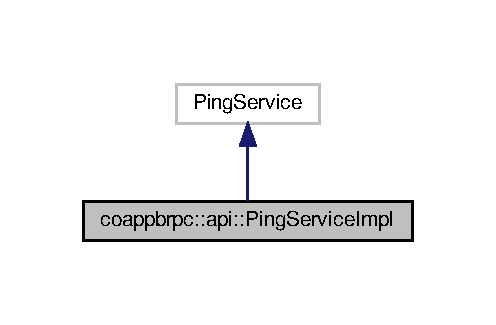
\includegraphics[width=238pt]{classcoappbrpc_1_1api_1_1PingServiceImpl__inherit__graph}
\end{center}
\end{figure}


Collaboration diagram for coappbrpc\+:\+:api\+:\+:Ping\+Service\+Impl\+:
\nopagebreak
\begin{figure}[H]
\begin{center}
\leavevmode
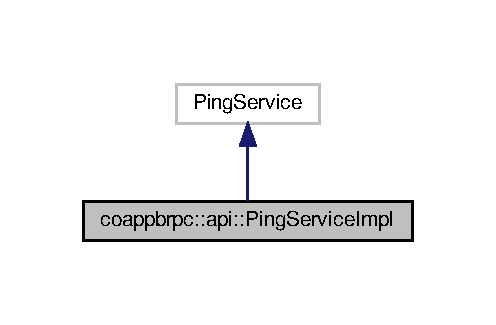
\includegraphics[width=238pt]{classcoappbrpc_1_1api_1_1PingServiceImpl__coll__graph}
\end{center}
\end{figure}
\subsection*{Public Member Functions}
\begin{DoxyCompactItemize}
\item 
\mbox{\Hypertarget{classcoappbrpc_1_1api_1_1PingServiceImpl_ad0fdead8e69607ba9114b277fe96844b}\label{classcoappbrpc_1_1api_1_1PingServiceImpl_ad0fdead8e69607ba9114b277fe96844b}} 
virtual void {\bfseries Ping} (Rpc\+Controller $\ast$controller, const Ping\+Request $\ast$request, Ping\+Response $\ast$response, Closure $\ast$done)
\end{DoxyCompactItemize}


The documentation for this class was generated from the following file\+:\begin{DoxyCompactItemize}
\item 
example/ping/server.\+cpp\end{DoxyCompactItemize}

\hypertarget{classcoappbrpc_1_1Request}{}\section{coappbrpc\+:\+:Request Class Reference}
\label{classcoappbrpc_1_1Request}\index{coappbrpc\+::\+Request@{coappbrpc\+::\+Request}}


Inheritance diagram for coappbrpc\+:\+:Request\+:
% FIG 0


Collaboration diagram for coappbrpc\+:\+:Request\+:
% FIG 1
\subsection*{Classes}
\begin{DoxyCompactItemize}
\item 
class \hyperlink{classcoappbrpc_1_1Request_1_1HasBitSetters}{Has\+Bit\+Setters}
\end{DoxyCompactItemize}
\subsection*{Public Member Functions}
\begin{DoxyCompactItemize}
\item 
\mbox{\Hypertarget{classcoappbrpc_1_1Request_a47a39167c3ce45e3c3fd7e02b1fc543d}\label{classcoappbrpc_1_1Request_a47a39167c3ce45e3c3fd7e02b1fc543d}} 
{\bfseries Request} (const \hyperlink{classcoappbrpc_1_1Request}{Request} \&from)
\item 
\mbox{\Hypertarget{classcoappbrpc_1_1Request_a16ffbdf9dda710d5118fa74bac52d61a}\label{classcoappbrpc_1_1Request_a16ffbdf9dda710d5118fa74bac52d61a}} 
\hyperlink{classcoappbrpc_1_1Request}{Request} \& {\bfseries operator=} (const \hyperlink{classcoappbrpc_1_1Request}{Request} \&from)
\item 
\mbox{\Hypertarget{classcoappbrpc_1_1Request_a98653b1ed247cbb328495fe00c8741b1}\label{classcoappbrpc_1_1Request_a98653b1ed247cbb328495fe00c8741b1}} 
void {\bfseries Swap} (\hyperlink{classcoappbrpc_1_1Request}{Request} $\ast$other)
\item 
\mbox{\Hypertarget{classcoappbrpc_1_1Request_aeff1989d6f4b25ae7923492201489f75}\label{classcoappbrpc_1_1Request_aeff1989d6f4b25ae7923492201489f75}} 
\hyperlink{classcoappbrpc_1_1Request}{Request} $\ast$ {\bfseries New} () const final
\item 
\mbox{\Hypertarget{classcoappbrpc_1_1Request_a9b3c97de3afd1435da415cf623ca5a49}\label{classcoappbrpc_1_1Request_a9b3c97de3afd1435da415cf623ca5a49}} 
\hyperlink{classcoappbrpc_1_1Request}{Request} $\ast$ {\bfseries New} (\+::google\+::protobuf\+::\+Arena $\ast$arena) const final
\item 
\mbox{\Hypertarget{classcoappbrpc_1_1Request_a4d2f9d18648487a08edb25e1f9a6a4c2}\label{classcoappbrpc_1_1Request_a4d2f9d18648487a08edb25e1f9a6a4c2}} 
void {\bfseries Copy\+From} (const \+::google\+::protobuf\+::\+Message \&from) final
\item 
\mbox{\Hypertarget{classcoappbrpc_1_1Request_a74dcbf992d27f7d18822e381dac3713c}\label{classcoappbrpc_1_1Request_a74dcbf992d27f7d18822e381dac3713c}} 
void {\bfseries Merge\+From} (const \+::google\+::protobuf\+::\+Message \&from) final
\item 
\mbox{\Hypertarget{classcoappbrpc_1_1Request_a4c74f0343c8b770aab1074a3571ba9ce}\label{classcoappbrpc_1_1Request_a4c74f0343c8b770aab1074a3571ba9ce}} 
void {\bfseries Copy\+From} (const \hyperlink{classcoappbrpc_1_1Request}{Request} \&from)
\item 
\mbox{\Hypertarget{classcoappbrpc_1_1Request_a745157bc69afe4509e157ca9835e2d9c}\label{classcoappbrpc_1_1Request_a745157bc69afe4509e157ca9835e2d9c}} 
void {\bfseries Merge\+From} (const \hyperlink{classcoappbrpc_1_1Request}{Request} \&from)
\item 
\mbox{\Hypertarget{classcoappbrpc_1_1Request_a3699329574cf56b9b684dcb984176910}\label{classcoappbrpc_1_1Request_a3699329574cf56b9b684dcb984176910}} 
void {\bfseries Clear} () final
\item 
\mbox{\Hypertarget{classcoappbrpc_1_1Request_a3b3733fa1bb216ecaa3013b506485bf3}\label{classcoappbrpc_1_1Request_a3b3733fa1bb216ecaa3013b506485bf3}} 
bool {\bfseries Is\+Initialized} () const final
\item 
\mbox{\Hypertarget{classcoappbrpc_1_1Request_af3933a049ac9a8bcae6efeccb6be6823}\label{classcoappbrpc_1_1Request_af3933a049ac9a8bcae6efeccb6be6823}} 
size\+\_\+t {\bfseries Byte\+Size\+Long} () const final
\item 
\mbox{\Hypertarget{classcoappbrpc_1_1Request_a590deeb6a5bf95ab9e0bdbff4d6ed92a}\label{classcoappbrpc_1_1Request_a590deeb6a5bf95ab9e0bdbff4d6ed92a}} 
bool {\bfseries Merge\+Partial\+From\+Coded\+Stream} (\+::google\+::protobuf\+::io\+::\+Coded\+Input\+Stream $\ast$input) final
\item 
\mbox{\Hypertarget{classcoappbrpc_1_1Request_a707fec97351a1cf2e2af40c4628579a4}\label{classcoappbrpc_1_1Request_a707fec97351a1cf2e2af40c4628579a4}} 
void {\bfseries Serialize\+With\+Cached\+Sizes} (\+::google\+::protobuf\+::io\+::\+Coded\+Output\+Stream $\ast$output) const final
\item 
\mbox{\Hypertarget{classcoappbrpc_1_1Request_abf99985c08c4b47e71275959b2a5a643}\label{classcoappbrpc_1_1Request_abf99985c08c4b47e71275959b2a5a643}} 
\+::google\+::protobuf\+::uint8 $\ast$ {\bfseries Internal\+Serialize\+With\+Cached\+Sizes\+To\+Array} (bool deterministic, \+::google\+::protobuf\+::uint8 $\ast$target) const final
\item 
\mbox{\Hypertarget{classcoappbrpc_1_1Request_a3e6421e0c870ce79d40ad896db78d0c7}\label{classcoappbrpc_1_1Request_a3e6421e0c870ce79d40ad896db78d0c7}} 
int {\bfseries Get\+Cached\+Size} () const final
\item 
\mbox{\Hypertarget{classcoappbrpc_1_1Request_a09b5a02b3a1a5b62d9cc02e5861cebe4}\label{classcoappbrpc_1_1Request_a09b5a02b3a1a5b62d9cc02e5861cebe4}} 
\+::google\+::protobuf\+::\+Metadata {\bfseries Get\+Metadata} () const final
\item 
\mbox{\Hypertarget{classcoappbrpc_1_1Request_a9ede440fd8f0d845e4fe8ce1deb5973f}\label{classcoappbrpc_1_1Request_a9ede440fd8f0d845e4fe8ce1deb5973f}} 
void {\bfseries clear\+\_\+version} ()
\item 
\mbox{\Hypertarget{classcoappbrpc_1_1Request_a35f5cd80696f6c7b56c4d4e24d1f344a}\label{classcoappbrpc_1_1Request_a35f5cd80696f6c7b56c4d4e24d1f344a}} 
const \+::std\+::string \& {\bfseries version} () const
\item 
\mbox{\Hypertarget{classcoappbrpc_1_1Request_a6563f82b332ac0714c61daa2ad010374}\label{classcoappbrpc_1_1Request_a6563f82b332ac0714c61daa2ad010374}} 
void {\bfseries set\+\_\+version} (const \+::std\+::string \&value)
\item 
\mbox{\Hypertarget{classcoappbrpc_1_1Request_ad431e4dc189a9e3ebe32b5d058727b69}\label{classcoappbrpc_1_1Request_ad431e4dc189a9e3ebe32b5d058727b69}} 
void {\bfseries set\+\_\+version} (const char $\ast$value)
\item 
\mbox{\Hypertarget{classcoappbrpc_1_1Request_a3111278b77ba1c4b5b1531df140124f2}\label{classcoappbrpc_1_1Request_a3111278b77ba1c4b5b1531df140124f2}} 
void {\bfseries set\+\_\+version} (const char $\ast$value, size\+\_\+t size)
\item 
\mbox{\Hypertarget{classcoappbrpc_1_1Request_ae9ec424b715eace57f2d6dc7d500f286}\label{classcoappbrpc_1_1Request_ae9ec424b715eace57f2d6dc7d500f286}} 
\+::std\+::string $\ast$ {\bfseries mutable\+\_\+version} ()
\item 
\mbox{\Hypertarget{classcoappbrpc_1_1Request_a06f0d58dc46d2fae775c5dfdc71458be}\label{classcoappbrpc_1_1Request_a06f0d58dc46d2fae775c5dfdc71458be}} 
\+::std\+::string $\ast$ {\bfseries release\+\_\+version} ()
\item 
\mbox{\Hypertarget{classcoappbrpc_1_1Request_a6b06bcc01a30ab256cf15dd18089eeab}\label{classcoappbrpc_1_1Request_a6b06bcc01a30ab256cf15dd18089eeab}} 
void {\bfseries set\+\_\+allocated\+\_\+version} (\+::std\+::string $\ast$version)
\item 
\mbox{\Hypertarget{classcoappbrpc_1_1Request_a0fc178adfb20c19e00eeaab82b80f53f}\label{classcoappbrpc_1_1Request_a0fc178adfb20c19e00eeaab82b80f53f}} 
void {\bfseries clear\+\_\+service} ()
\item 
\mbox{\Hypertarget{classcoappbrpc_1_1Request_a7ad2daa87ccc004815226d499e958413}\label{classcoappbrpc_1_1Request_a7ad2daa87ccc004815226d499e958413}} 
const \+::std\+::string \& {\bfseries service} () const
\item 
\mbox{\Hypertarget{classcoappbrpc_1_1Request_afeac2f99fef1585356a8f3ac97b0f75e}\label{classcoappbrpc_1_1Request_afeac2f99fef1585356a8f3ac97b0f75e}} 
void {\bfseries set\+\_\+service} (const \+::std\+::string \&value)
\item 
\mbox{\Hypertarget{classcoappbrpc_1_1Request_a36bacf2f08ded736916657c94b14fc60}\label{classcoappbrpc_1_1Request_a36bacf2f08ded736916657c94b14fc60}} 
void {\bfseries set\+\_\+service} (const char $\ast$value)
\item 
\mbox{\Hypertarget{classcoappbrpc_1_1Request_aa59b8a2db7fcf08849232a23d90260d0}\label{classcoappbrpc_1_1Request_aa59b8a2db7fcf08849232a23d90260d0}} 
void {\bfseries set\+\_\+service} (const char $\ast$value, size\+\_\+t size)
\item 
\mbox{\Hypertarget{classcoappbrpc_1_1Request_a9fb0e2a179f69ad34a07025789a000d5}\label{classcoappbrpc_1_1Request_a9fb0e2a179f69ad34a07025789a000d5}} 
\+::std\+::string $\ast$ {\bfseries mutable\+\_\+service} ()
\item 
\mbox{\Hypertarget{classcoappbrpc_1_1Request_ad24c1c227bf3b8bd1c2ee60c3617eb7c}\label{classcoappbrpc_1_1Request_ad24c1c227bf3b8bd1c2ee60c3617eb7c}} 
\+::std\+::string $\ast$ {\bfseries release\+\_\+service} ()
\item 
\mbox{\Hypertarget{classcoappbrpc_1_1Request_a59e8d08d63e9f91ea83cad31d73ae7e6}\label{classcoappbrpc_1_1Request_a59e8d08d63e9f91ea83cad31d73ae7e6}} 
void {\bfseries set\+\_\+allocated\+\_\+service} (\+::std\+::string $\ast$service)
\item 
\mbox{\Hypertarget{classcoappbrpc_1_1Request_a0bf017c8c04f9ba6c9008d56ea417e70}\label{classcoappbrpc_1_1Request_a0bf017c8c04f9ba6c9008d56ea417e70}} 
void {\bfseries clear\+\_\+method} ()
\item 
\mbox{\Hypertarget{classcoappbrpc_1_1Request_a0fd5b103c1ce2681040a80f88fdb8b37}\label{classcoappbrpc_1_1Request_a0fd5b103c1ce2681040a80f88fdb8b37}} 
const \+::std\+::string \& {\bfseries method} () const
\item 
\mbox{\Hypertarget{classcoappbrpc_1_1Request_abce4c7d94de659fe0b1078907fade489}\label{classcoappbrpc_1_1Request_abce4c7d94de659fe0b1078907fade489}} 
void {\bfseries set\+\_\+method} (const \+::std\+::string \&value)
\item 
\mbox{\Hypertarget{classcoappbrpc_1_1Request_a578f6f991711590b9c55e17581f8561c}\label{classcoappbrpc_1_1Request_a578f6f991711590b9c55e17581f8561c}} 
void {\bfseries set\+\_\+method} (const char $\ast$value)
\item 
\mbox{\Hypertarget{classcoappbrpc_1_1Request_abb7aa04c7773dedb82e60d5569f3aa78}\label{classcoappbrpc_1_1Request_abb7aa04c7773dedb82e60d5569f3aa78}} 
void {\bfseries set\+\_\+method} (const char $\ast$value, size\+\_\+t size)
\item 
\mbox{\Hypertarget{classcoappbrpc_1_1Request_a1145ab28351a4c3f8dd846ce17770730}\label{classcoappbrpc_1_1Request_a1145ab28351a4c3f8dd846ce17770730}} 
\+::std\+::string $\ast$ {\bfseries mutable\+\_\+method} ()
\item 
\mbox{\Hypertarget{classcoappbrpc_1_1Request_a2394d4827b0c92238294c38424590419}\label{classcoappbrpc_1_1Request_a2394d4827b0c92238294c38424590419}} 
\+::std\+::string $\ast$ {\bfseries release\+\_\+method} ()
\item 
\mbox{\Hypertarget{classcoappbrpc_1_1Request_abc69e31e8d9b71ad106e57386d14891d}\label{classcoappbrpc_1_1Request_abc69e31e8d9b71ad106e57386d14891d}} 
void {\bfseries set\+\_\+allocated\+\_\+method} (\+::std\+::string $\ast$method)
\item 
\mbox{\Hypertarget{classcoappbrpc_1_1Request_a80b1ab7b95c197b7d7c7ef01d478d5c9}\label{classcoappbrpc_1_1Request_a80b1ab7b95c197b7d7c7ef01d478d5c9}} 
void {\bfseries clear\+\_\+params} ()
\item 
\mbox{\Hypertarget{classcoappbrpc_1_1Request_a475de4a3d35e86c91adad2b824bbd52d}\label{classcoappbrpc_1_1Request_a475de4a3d35e86c91adad2b824bbd52d}} 
const \+::std\+::string \& {\bfseries params} () const
\item 
\mbox{\Hypertarget{classcoappbrpc_1_1Request_a738278b90cadfe2e5452ade21fd34691}\label{classcoappbrpc_1_1Request_a738278b90cadfe2e5452ade21fd34691}} 
void {\bfseries set\+\_\+params} (const \+::std\+::string \&value)
\item 
\mbox{\Hypertarget{classcoappbrpc_1_1Request_a37741785a7e7ea8498839962a575d319}\label{classcoappbrpc_1_1Request_a37741785a7e7ea8498839962a575d319}} 
void {\bfseries set\+\_\+params} (const char $\ast$value)
\item 
\mbox{\Hypertarget{classcoappbrpc_1_1Request_a9fcffc4c495208606973bc8b6683248d}\label{classcoappbrpc_1_1Request_a9fcffc4c495208606973bc8b6683248d}} 
void {\bfseries set\+\_\+params} (const void $\ast$value, size\+\_\+t size)
\item 
\mbox{\Hypertarget{classcoappbrpc_1_1Request_a42c21d76e979369b8df159a1b1b03573}\label{classcoappbrpc_1_1Request_a42c21d76e979369b8df159a1b1b03573}} 
\+::std\+::string $\ast$ {\bfseries mutable\+\_\+params} ()
\item 
\mbox{\Hypertarget{classcoappbrpc_1_1Request_a2aec9643c67b70935692a3648af508aa}\label{classcoappbrpc_1_1Request_a2aec9643c67b70935692a3648af508aa}} 
\+::std\+::string $\ast$ {\bfseries release\+\_\+params} ()
\item 
\mbox{\Hypertarget{classcoappbrpc_1_1Request_aa7f19fbcc325f288b0d70b3e3eb55829}\label{classcoappbrpc_1_1Request_aa7f19fbcc325f288b0d70b3e3eb55829}} 
void {\bfseries set\+\_\+allocated\+\_\+params} (\+::std\+::string $\ast$params)
\item 
\mbox{\Hypertarget{classcoappbrpc_1_1Request_a687f7932f9718823e114a934d5d4a41f}\label{classcoappbrpc_1_1Request_a687f7932f9718823e114a934d5d4a41f}} 
void {\bfseries clear\+\_\+id} ()
\item 
\mbox{\Hypertarget{classcoappbrpc_1_1Request_a48a39437866e9a8f9ee50759966cbc7e}\label{classcoappbrpc_1_1Request_a48a39437866e9a8f9ee50759966cbc7e}} 
\+::google\+::protobuf\+::int32 {\bfseries id} () const
\item 
\mbox{\Hypertarget{classcoappbrpc_1_1Request_a6d5f7f9cbd2757ff922ed6339055dc5b}\label{classcoappbrpc_1_1Request_a6d5f7f9cbd2757ff922ed6339055dc5b}} 
void {\bfseries set\+\_\+id} (\+::google\+::protobuf\+::int32 value)
\end{DoxyCompactItemize}
\subsection*{Static Public Member Functions}
\begin{DoxyCompactItemize}
\item 
\mbox{\Hypertarget{classcoappbrpc_1_1Request_acee20e2a177227b514ff52c82cc23cdf}\label{classcoappbrpc_1_1Request_acee20e2a177227b514ff52c82cc23cdf}} 
static const \+::google\+::protobuf\+::\+Descriptor $\ast$ {\bfseries descriptor} ()
\item 
\mbox{\Hypertarget{classcoappbrpc_1_1Request_a24d20d232627a8baaf01bb0ed9266c46}\label{classcoappbrpc_1_1Request_a24d20d232627a8baaf01bb0ed9266c46}} 
static const \hyperlink{classcoappbrpc_1_1Request}{Request} \& {\bfseries default\+\_\+instance} ()
\item 
\mbox{\Hypertarget{classcoappbrpc_1_1Request_aa650d4a3da3187eb70e13f0d7931bad6}\label{classcoappbrpc_1_1Request_aa650d4a3da3187eb70e13f0d7931bad6}} 
static void {\bfseries Init\+As\+Default\+Instance} ()
\item 
\mbox{\Hypertarget{classcoappbrpc_1_1Request_a6f72b785009d065f41981a2a7ad8f294}\label{classcoappbrpc_1_1Request_a6f72b785009d065f41981a2a7ad8f294}} 
static const \hyperlink{classcoappbrpc_1_1Request}{Request} $\ast$ {\bfseries internal\+\_\+default\+\_\+instance} ()
\end{DoxyCompactItemize}
\subsection*{Static Public Attributes}
\begin{DoxyCompactItemize}
\item 
static constexpr int {\bfseries k\+Index\+In\+File\+Messages}
\item 
\mbox{\Hypertarget{classcoappbrpc_1_1Request_a6b131649a4743ce2e4d49c760c872d9a}\label{classcoappbrpc_1_1Request_a6b131649a4743ce2e4d49c760c872d9a}} 
static const int {\bfseries k\+Version\+Field\+Number} = 1
\item 
\mbox{\Hypertarget{classcoappbrpc_1_1Request_a99a19c8f4f9a2a2a336205fc58054ff7}\label{classcoappbrpc_1_1Request_a99a19c8f4f9a2a2a336205fc58054ff7}} 
static const int {\bfseries k\+Service\+Field\+Number} = 2
\item 
\mbox{\Hypertarget{classcoappbrpc_1_1Request_a3a65833e8c31413fcfd80a10762aa42a}\label{classcoappbrpc_1_1Request_a3a65833e8c31413fcfd80a10762aa42a}} 
static const int {\bfseries k\+Method\+Field\+Number} = 3
\item 
\mbox{\Hypertarget{classcoappbrpc_1_1Request_a47ecf8c271e621d08fa508e7364a19dd}\label{classcoappbrpc_1_1Request_a47ecf8c271e621d08fa508e7364a19dd}} 
static const int {\bfseries k\+Params\+Field\+Number} = 4
\item 
\mbox{\Hypertarget{classcoappbrpc_1_1Request_aa3808ae5825a8d4b9bfd587b63db6325}\label{classcoappbrpc_1_1Request_aa3808ae5825a8d4b9bfd587b63db6325}} 
static const int {\bfseries k\+Id\+Field\+Number} = 5
\end{DoxyCompactItemize}
\subsection*{Friends}
\begin{DoxyCompactItemize}
\item 
\mbox{\Hypertarget{classcoappbrpc_1_1Request_a65c087bf06ded9c9be363691f7b7bafa}\label{classcoappbrpc_1_1Request_a65c087bf06ded9c9be363691f7b7bafa}} 
struct {\bfseries \+::\+Table\+Struct\+\_\+\+Msg\+Schema\+\_\+2eproto}
\item 
\mbox{\Hypertarget{classcoappbrpc_1_1Request_ad4e2154e85b9878aaaf70f5f9afde893}\label{classcoappbrpc_1_1Request_ad4e2154e85b9878aaaf70f5f9afde893}} 
void {\bfseries swap} (\hyperlink{classcoappbrpc_1_1Request}{Request} \&a, \hyperlink{classcoappbrpc_1_1Request}{Request} \&b)
\end{DoxyCompactItemize}


\subsection{Member Data Documentation}
\mbox{\Hypertarget{classcoappbrpc_1_1Request_a20c30089794b648d7e2f0d9ad193c625}\label{classcoappbrpc_1_1Request_a20c30089794b648d7e2f0d9ad193c625}} 
\index{coappbrpc\+::\+Request@{coappbrpc\+::\+Request}!k\+Index\+In\+File\+Messages@{k\+Index\+In\+File\+Messages}}
\index{k\+Index\+In\+File\+Messages@{k\+Index\+In\+File\+Messages}!coappbrpc\+::\+Request@{coappbrpc\+::\+Request}}
\subsubsection{\texorpdfstring{k\+Index\+In\+File\+Messages}{kIndexInFileMessages}}
{\footnotesize\ttfamily constexpr int coappbrpc\+::\+Request\+::k\+Index\+In\+File\+Messages\hspace{0.3cm}{\ttfamily [static]}}

{\bfseries Initial value\+:}
\begin{DoxyCode}
=
    0
\end{DoxyCode}


The documentation for this class was generated from the following files\+:\begin{DoxyCompactItemize}
\item 
build/proto/Msg\+Schema.\+pb.\+h\item 
build/proto/Msg\+Schema.\+pb.\+cc\end{DoxyCompactItemize}

\hypertarget{classcoappbrpc_1_1RequestDefaultTypeInternal}{}\section{coappbrpc\+:\+:Request\+Default\+Type\+Internal Class Reference}
\label{classcoappbrpc_1_1RequestDefaultTypeInternal}\index{coappbrpc\+::\+Request\+Default\+Type\+Internal@{coappbrpc\+::\+Request\+Default\+Type\+Internal}}
\subsection*{Public Attributes}
\begin{DoxyCompactItemize}
\item 
\mbox{\Hypertarget{classcoappbrpc_1_1RequestDefaultTypeInternal_a9e4ffe30bd0910a694598331fb695828}\label{classcoappbrpc_1_1RequestDefaultTypeInternal_a9e4ffe30bd0910a694598331fb695828}} 
\+::google\+::protobuf\+::internal\+::\+Explicitly\+Constructed$<$ \hyperlink{classcoappbrpc_1_1Request}{Request} $>$ {\bfseries \+\_\+instance}
\end{DoxyCompactItemize}


The documentation for this class was generated from the following file\+:\begin{DoxyCompactItemize}
\item 
build/proto/Msg\+Schema.\+pb.\+cc\end{DoxyCompactItemize}

\hypertarget{classcoappbrpc_1_1Response}{}\section{coappbrpc\+:\+:Response Class Reference}
\label{classcoappbrpc_1_1Response}\index{coappbrpc\+::\+Response@{coappbrpc\+::\+Response}}


Inheritance diagram for coappbrpc\+:\+:Response\+:\nopagebreak
\begin{figure}[H]
\begin{center}
\leavevmode
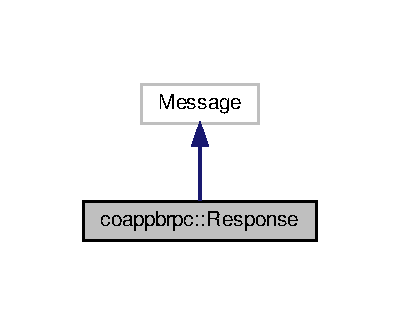
\includegraphics[width=192pt]{classcoappbrpc_1_1Response__inherit__graph}
\end{center}
\end{figure}


Collaboration diagram for coappbrpc\+:\+:Response\+:\nopagebreak
\begin{figure}[H]
\begin{center}
\leavevmode
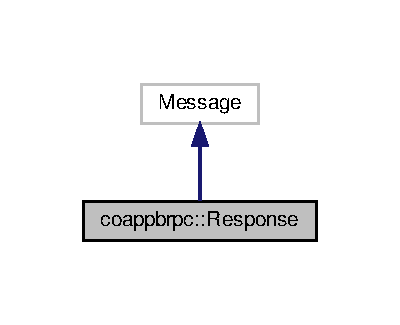
\includegraphics[width=192pt]{classcoappbrpc_1_1Response__coll__graph}
\end{center}
\end{figure}
\subsection*{Classes}
\begin{DoxyCompactItemize}
\item 
class \hyperlink{classcoappbrpc_1_1Response_1_1HasBitSetters}{Has\+Bit\+Setters}
\end{DoxyCompactItemize}
\subsection*{Public Member Functions}
\begin{DoxyCompactItemize}
\item 
\mbox{\Hypertarget{classcoappbrpc_1_1Response_a24904bb0f0787fce30908baa49edc716}\label{classcoappbrpc_1_1Response_a24904bb0f0787fce30908baa49edc716}} 
{\bfseries Response} (const \hyperlink{classcoappbrpc_1_1Response}{Response} \&from)
\item 
\mbox{\Hypertarget{classcoappbrpc_1_1Response_a61b7fa1a0db69410c56d5fe68780c672}\label{classcoappbrpc_1_1Response_a61b7fa1a0db69410c56d5fe68780c672}} 
\hyperlink{classcoappbrpc_1_1Response}{Response} \& {\bfseries operator=} (const \hyperlink{classcoappbrpc_1_1Response}{Response} \&from)
\item 
\mbox{\Hypertarget{classcoappbrpc_1_1Response_a8c4a23436a8b69a56ae78b77275b6c73}\label{classcoappbrpc_1_1Response_a8c4a23436a8b69a56ae78b77275b6c73}} 
void {\bfseries Swap} (\hyperlink{classcoappbrpc_1_1Response}{Response} $\ast$other)
\item 
\mbox{\Hypertarget{classcoappbrpc_1_1Response_a5376077cc9b1c06db82f865bbdde3393}\label{classcoappbrpc_1_1Response_a5376077cc9b1c06db82f865bbdde3393}} 
\hyperlink{classcoappbrpc_1_1Response}{Response} $\ast$ {\bfseries New} () const final
\item 
\mbox{\Hypertarget{classcoappbrpc_1_1Response_abd3c0c6327b76e29a6346ed2c4a3a799}\label{classcoappbrpc_1_1Response_abd3c0c6327b76e29a6346ed2c4a3a799}} 
\hyperlink{classcoappbrpc_1_1Response}{Response} $\ast$ {\bfseries New} (\+::google\+::protobuf\+::\+Arena $\ast$arena) const final
\item 
\mbox{\Hypertarget{classcoappbrpc_1_1Response_acd3ee1f81b27d08c0ffb155bdb9b3c1d}\label{classcoappbrpc_1_1Response_acd3ee1f81b27d08c0ffb155bdb9b3c1d}} 
void {\bfseries Copy\+From} (const \+::google\+::protobuf\+::\+Message \&from) final
\item 
\mbox{\Hypertarget{classcoappbrpc_1_1Response_ad20d2e5d879b0a4d6cd313b4da6618a1}\label{classcoappbrpc_1_1Response_ad20d2e5d879b0a4d6cd313b4da6618a1}} 
void {\bfseries Merge\+From} (const \+::google\+::protobuf\+::\+Message \&from) final
\item 
\mbox{\Hypertarget{classcoappbrpc_1_1Response_a3a27916c27b9cf8e3a437d1cbd1147c4}\label{classcoappbrpc_1_1Response_a3a27916c27b9cf8e3a437d1cbd1147c4}} 
void {\bfseries Copy\+From} (const \hyperlink{classcoappbrpc_1_1Response}{Response} \&from)
\item 
\mbox{\Hypertarget{classcoappbrpc_1_1Response_a9e65ff105d739a4f0fda6cf8ea0dd91f}\label{classcoappbrpc_1_1Response_a9e65ff105d739a4f0fda6cf8ea0dd91f}} 
void {\bfseries Merge\+From} (const \hyperlink{classcoappbrpc_1_1Response}{Response} \&from)
\item 
\mbox{\Hypertarget{classcoappbrpc_1_1Response_aa9b68b199f18a06cf3036430e6469ec2}\label{classcoappbrpc_1_1Response_aa9b68b199f18a06cf3036430e6469ec2}} 
void {\bfseries Clear} () final
\item 
\mbox{\Hypertarget{classcoappbrpc_1_1Response_a687c386d4428e724be5226c2c2c14479}\label{classcoappbrpc_1_1Response_a687c386d4428e724be5226c2c2c14479}} 
bool {\bfseries Is\+Initialized} () const final
\item 
\mbox{\Hypertarget{classcoappbrpc_1_1Response_a85bd1f7ae73c9dc3d370547a2794d56d}\label{classcoappbrpc_1_1Response_a85bd1f7ae73c9dc3d370547a2794d56d}} 
size\+\_\+t {\bfseries Byte\+Size\+Long} () const final
\item 
\mbox{\Hypertarget{classcoappbrpc_1_1Response_a338f6e91d6b68734fab073e37e842104}\label{classcoappbrpc_1_1Response_a338f6e91d6b68734fab073e37e842104}} 
bool {\bfseries Merge\+Partial\+From\+Coded\+Stream} (\+::google\+::protobuf\+::io\+::\+Coded\+Input\+Stream $\ast$input) final
\item 
\mbox{\Hypertarget{classcoappbrpc_1_1Response_a9245b3575fed37198c288936a47ba31c}\label{classcoappbrpc_1_1Response_a9245b3575fed37198c288936a47ba31c}} 
void {\bfseries Serialize\+With\+Cached\+Sizes} (\+::google\+::protobuf\+::io\+::\+Coded\+Output\+Stream $\ast$output) const final
\item 
\mbox{\Hypertarget{classcoappbrpc_1_1Response_a54352ac27422f88aec17253468593172}\label{classcoappbrpc_1_1Response_a54352ac27422f88aec17253468593172}} 
\+::google\+::protobuf\+::uint8 $\ast$ {\bfseries Internal\+Serialize\+With\+Cached\+Sizes\+To\+Array} (bool deterministic, \+::google\+::protobuf\+::uint8 $\ast$target) const final
\item 
\mbox{\Hypertarget{classcoappbrpc_1_1Response_a4eeebf1befe309f178185e3f8b4da3d1}\label{classcoappbrpc_1_1Response_a4eeebf1befe309f178185e3f8b4da3d1}} 
int {\bfseries Get\+Cached\+Size} () const final
\item 
\mbox{\Hypertarget{classcoappbrpc_1_1Response_a6724cea13f3ebabd4db02fead5bf0b12}\label{classcoappbrpc_1_1Response_a6724cea13f3ebabd4db02fead5bf0b12}} 
\+::google\+::protobuf\+::\+Metadata {\bfseries Get\+Metadata} () const final
\item 
\mbox{\Hypertarget{classcoappbrpc_1_1Response_a56714ff4c70fe010ca24ee2ab7c08b5a}\label{classcoappbrpc_1_1Response_a56714ff4c70fe010ca24ee2ab7c08b5a}} 
void {\bfseries clear\+\_\+version} ()
\item 
\mbox{\Hypertarget{classcoappbrpc_1_1Response_accf32df398527b83ac819ad6ddeb6bdf}\label{classcoappbrpc_1_1Response_accf32df398527b83ac819ad6ddeb6bdf}} 
const \+::std\+::string \& {\bfseries version} () const
\item 
\mbox{\Hypertarget{classcoappbrpc_1_1Response_a68bd09f954ddf08a00d478735e1c1eae}\label{classcoappbrpc_1_1Response_a68bd09f954ddf08a00d478735e1c1eae}} 
void {\bfseries set\+\_\+version} (const \+::std\+::string \&value)
\item 
\mbox{\Hypertarget{classcoappbrpc_1_1Response_a573b1dd1a43e6b6b6ad96a964ab576bb}\label{classcoappbrpc_1_1Response_a573b1dd1a43e6b6b6ad96a964ab576bb}} 
void {\bfseries set\+\_\+version} (const char $\ast$value)
\item 
\mbox{\Hypertarget{classcoappbrpc_1_1Response_aef97211cb8eebdef5b706d371098c9fe}\label{classcoappbrpc_1_1Response_aef97211cb8eebdef5b706d371098c9fe}} 
void {\bfseries set\+\_\+version} (const char $\ast$value, size\+\_\+t size)
\item 
\mbox{\Hypertarget{classcoappbrpc_1_1Response_a41691f43bfc03b7bd5703cc79a2e70a1}\label{classcoappbrpc_1_1Response_a41691f43bfc03b7bd5703cc79a2e70a1}} 
\+::std\+::string $\ast$ {\bfseries mutable\+\_\+version} ()
\item 
\mbox{\Hypertarget{classcoappbrpc_1_1Response_aab3845a6fca89242d3a507f1fb4ef411}\label{classcoappbrpc_1_1Response_aab3845a6fca89242d3a507f1fb4ef411}} 
\+::std\+::string $\ast$ {\bfseries release\+\_\+version} ()
\item 
\mbox{\Hypertarget{classcoappbrpc_1_1Response_a0f7068126473cbac403752d3be8c4374}\label{classcoappbrpc_1_1Response_a0f7068126473cbac403752d3be8c4374}} 
void {\bfseries set\+\_\+allocated\+\_\+version} (\+::std\+::string $\ast$version)
\item 
\mbox{\Hypertarget{classcoappbrpc_1_1Response_af8a767aac84ca69eb13656e15138fe77}\label{classcoappbrpc_1_1Response_af8a767aac84ca69eb13656e15138fe77}} 
void {\bfseries clear\+\_\+result} ()
\item 
\mbox{\Hypertarget{classcoappbrpc_1_1Response_a4a917b0e205dc60bf1a5d424fa5c4728}\label{classcoappbrpc_1_1Response_a4a917b0e205dc60bf1a5d424fa5c4728}} 
const \+::std\+::string \& {\bfseries result} () const
\item 
\mbox{\Hypertarget{classcoappbrpc_1_1Response_a4181db1a6c4b74f734693689d60d2edc}\label{classcoappbrpc_1_1Response_a4181db1a6c4b74f734693689d60d2edc}} 
void {\bfseries set\+\_\+result} (const \+::std\+::string \&value)
\item 
\mbox{\Hypertarget{classcoappbrpc_1_1Response_a232e7faf993df8c3c3adf40395091353}\label{classcoappbrpc_1_1Response_a232e7faf993df8c3c3adf40395091353}} 
void {\bfseries set\+\_\+result} (const char $\ast$value)
\item 
\mbox{\Hypertarget{classcoappbrpc_1_1Response_a6869735924f8020db2c8edf16ffea9a3}\label{classcoappbrpc_1_1Response_a6869735924f8020db2c8edf16ffea9a3}} 
void {\bfseries set\+\_\+result} (const void $\ast$value, size\+\_\+t size)
\item 
\mbox{\Hypertarget{classcoappbrpc_1_1Response_a3023ea3c2231705bd8ebd4754a0dd5aa}\label{classcoappbrpc_1_1Response_a3023ea3c2231705bd8ebd4754a0dd5aa}} 
\+::std\+::string $\ast$ {\bfseries mutable\+\_\+result} ()
\item 
\mbox{\Hypertarget{classcoappbrpc_1_1Response_ae35bcc72629ab642c373f331533d1ada}\label{classcoappbrpc_1_1Response_ae35bcc72629ab642c373f331533d1ada}} 
\+::std\+::string $\ast$ {\bfseries release\+\_\+result} ()
\item 
\mbox{\Hypertarget{classcoappbrpc_1_1Response_a3c01ab6b32b7411301538f447c1bc532}\label{classcoappbrpc_1_1Response_a3c01ab6b32b7411301538f447c1bc532}} 
void {\bfseries set\+\_\+allocated\+\_\+result} (\+::std\+::string $\ast$result)
\item 
\mbox{\Hypertarget{classcoappbrpc_1_1Response_a6a51678205f747030d38bfef138d705e}\label{classcoappbrpc_1_1Response_a6a51678205f747030d38bfef138d705e}} 
bool {\bfseries has\+\_\+error} () const
\item 
\mbox{\Hypertarget{classcoappbrpc_1_1Response_ac226b43c4a08c6fcb8b68d68c20b60ab}\label{classcoappbrpc_1_1Response_ac226b43c4a08c6fcb8b68d68c20b60ab}} 
void {\bfseries clear\+\_\+error} ()
\item 
\mbox{\Hypertarget{classcoappbrpc_1_1Response_a42b9742feb5e666028ef646e1854523f}\label{classcoappbrpc_1_1Response_a42b9742feb5e666028ef646e1854523f}} 
const \+::\hyperlink{classcoappbrpc_1_1Error}{coappbrpc\+::\+Error} \& {\bfseries error} () const
\item 
\mbox{\Hypertarget{classcoappbrpc_1_1Response_a024c37fee8ee34f3daaa45ff55d39e84}\label{classcoappbrpc_1_1Response_a024c37fee8ee34f3daaa45ff55d39e84}} 
\+::\hyperlink{classcoappbrpc_1_1Error}{coappbrpc\+::\+Error} $\ast$ {\bfseries release\+\_\+error} ()
\item 
\mbox{\Hypertarget{classcoappbrpc_1_1Response_a48c1ac0df3977860dd2531d6c8429ad9}\label{classcoappbrpc_1_1Response_a48c1ac0df3977860dd2531d6c8429ad9}} 
\+::\hyperlink{classcoappbrpc_1_1Error}{coappbrpc\+::\+Error} $\ast$ {\bfseries mutable\+\_\+error} ()
\item 
\mbox{\Hypertarget{classcoappbrpc_1_1Response_aa536601e1f7dcd45fd6fccffa6e15ca9}\label{classcoappbrpc_1_1Response_aa536601e1f7dcd45fd6fccffa6e15ca9}} 
void {\bfseries set\+\_\+allocated\+\_\+error} (\+::\hyperlink{classcoappbrpc_1_1Error}{coappbrpc\+::\+Error} $\ast$error)
\item 
\mbox{\Hypertarget{classcoappbrpc_1_1Response_a205de4d84232bde24326a6274d9b8acf}\label{classcoappbrpc_1_1Response_a205de4d84232bde24326a6274d9b8acf}} 
void {\bfseries clear\+\_\+id} ()
\item 
\mbox{\Hypertarget{classcoappbrpc_1_1Response_a89389be177aab69c762aaf218821bb32}\label{classcoappbrpc_1_1Response_a89389be177aab69c762aaf218821bb32}} 
\+::google\+::protobuf\+::int32 {\bfseries id} () const
\item 
\mbox{\Hypertarget{classcoappbrpc_1_1Response_af23aeab5cc0df75a26500f87e9942cee}\label{classcoappbrpc_1_1Response_af23aeab5cc0df75a26500f87e9942cee}} 
void {\bfseries set\+\_\+id} (\+::google\+::protobuf\+::int32 value)
\end{DoxyCompactItemize}
\subsection*{Static Public Member Functions}
\begin{DoxyCompactItemize}
\item 
\mbox{\Hypertarget{classcoappbrpc_1_1Response_aee7d5c409330433ba6061269965d7dd5}\label{classcoappbrpc_1_1Response_aee7d5c409330433ba6061269965d7dd5}} 
static const \+::google\+::protobuf\+::\+Descriptor $\ast$ {\bfseries descriptor} ()
\item 
\mbox{\Hypertarget{classcoappbrpc_1_1Response_a61ecfdb459c74f3ce536b878d5759007}\label{classcoappbrpc_1_1Response_a61ecfdb459c74f3ce536b878d5759007}} 
static const \hyperlink{classcoappbrpc_1_1Response}{Response} \& {\bfseries default\+\_\+instance} ()
\item 
\mbox{\Hypertarget{classcoappbrpc_1_1Response_a07665b433b0600546098d98a0afb52d7}\label{classcoappbrpc_1_1Response_a07665b433b0600546098d98a0afb52d7}} 
static void {\bfseries Init\+As\+Default\+Instance} ()
\item 
\mbox{\Hypertarget{classcoappbrpc_1_1Response_a0551fd997235f3871029b45c170b70ed}\label{classcoappbrpc_1_1Response_a0551fd997235f3871029b45c170b70ed}} 
static const \hyperlink{classcoappbrpc_1_1Response}{Response} $\ast$ {\bfseries internal\+\_\+default\+\_\+instance} ()
\end{DoxyCompactItemize}
\subsection*{Static Public Attributes}
\begin{DoxyCompactItemize}
\item 
static constexpr int {\bfseries k\+Index\+In\+File\+Messages}
\item 
\mbox{\Hypertarget{classcoappbrpc_1_1Response_a419e8532ffd97e6bab8cdcf27d31203f}\label{classcoappbrpc_1_1Response_a419e8532ffd97e6bab8cdcf27d31203f}} 
static const int {\bfseries k\+Version\+Field\+Number} = 1
\item 
\mbox{\Hypertarget{classcoappbrpc_1_1Response_a0132ee8e4087c92e607c548d46474964}\label{classcoappbrpc_1_1Response_a0132ee8e4087c92e607c548d46474964}} 
static const int {\bfseries k\+Result\+Field\+Number} = 2
\item 
\mbox{\Hypertarget{classcoappbrpc_1_1Response_ae7fdafbc86f89e117a6760c67eb3d9c2}\label{classcoappbrpc_1_1Response_ae7fdafbc86f89e117a6760c67eb3d9c2}} 
static const int {\bfseries k\+Error\+Field\+Number} = 3
\item 
\mbox{\Hypertarget{classcoappbrpc_1_1Response_ab1099b6e840365727c22e8bbe79f979a}\label{classcoappbrpc_1_1Response_ab1099b6e840365727c22e8bbe79f979a}} 
static const int {\bfseries k\+Id\+Field\+Number} = 4
\end{DoxyCompactItemize}
\subsection*{Friends}
\begin{DoxyCompactItemize}
\item 
\mbox{\Hypertarget{classcoappbrpc_1_1Response_a65c087bf06ded9c9be363691f7b7bafa}\label{classcoappbrpc_1_1Response_a65c087bf06ded9c9be363691f7b7bafa}} 
struct {\bfseries \+::\+Table\+Struct\+\_\+\+Msg\+Schema\+\_\+2eproto}
\item 
\mbox{\Hypertarget{classcoappbrpc_1_1Response_abd2d29760e9668486937c4d6f11784e6}\label{classcoappbrpc_1_1Response_abd2d29760e9668486937c4d6f11784e6}} 
void {\bfseries swap} (\hyperlink{classcoappbrpc_1_1Response}{Response} \&a, \hyperlink{classcoappbrpc_1_1Response}{Response} \&b)
\end{DoxyCompactItemize}


\subsection{Member Data Documentation}
\mbox{\Hypertarget{classcoappbrpc_1_1Response_ae8e167e80cc311e00980ac897decdceb}\label{classcoappbrpc_1_1Response_ae8e167e80cc311e00980ac897decdceb}} 
\index{coappbrpc\+::\+Response@{coappbrpc\+::\+Response}!k\+Index\+In\+File\+Messages@{k\+Index\+In\+File\+Messages}}
\index{k\+Index\+In\+File\+Messages@{k\+Index\+In\+File\+Messages}!coappbrpc\+::\+Response@{coappbrpc\+::\+Response}}
\subsubsection{\texorpdfstring{k\+Index\+In\+File\+Messages}{kIndexInFileMessages}}
{\footnotesize\ttfamily constexpr int coappbrpc\+::\+Response\+::k\+Index\+In\+File\+Messages\hspace{0.3cm}{\ttfamily [static]}}

{\bfseries Initial value\+:}
\begin{DoxyCode}
=
    2
\end{DoxyCode}


The documentation for this class was generated from the following files\+:\begin{DoxyCompactItemize}
\item 
build/proto/Msg\+Schema.\+pb.\+h\item 
build/proto/Msg\+Schema.\+pb.\+cc\end{DoxyCompactItemize}

\hypertarget{classcoappbrpc_1_1ResponseDefaultTypeInternal}{}\section{coappbrpc\+:\+:Response\+Default\+Type\+Internal Class Reference}
\label{classcoappbrpc_1_1ResponseDefaultTypeInternal}\index{coappbrpc\+::\+Response\+Default\+Type\+Internal@{coappbrpc\+::\+Response\+Default\+Type\+Internal}}
\subsection*{Public Attributes}
\begin{DoxyCompactItemize}
\item 
\mbox{\Hypertarget{classcoappbrpc_1_1ResponseDefaultTypeInternal_a2682abc1502e4594ce2ef83ca88e219d}\label{classcoappbrpc_1_1ResponseDefaultTypeInternal_a2682abc1502e4594ce2ef83ca88e219d}} 
\+::google\+::protobuf\+::internal\+::\+Explicitly\+Constructed$<$ \hyperlink{classcoappbrpc_1_1Response}{Response} $>$ {\bfseries \+\_\+instance}
\end{DoxyCompactItemize}


The documentation for this class was generated from the following file\+:\begin{DoxyCompactItemize}
\item 
build/proto/Msg\+Schema.\+pb.\+cc\end{DoxyCompactItemize}

\hypertarget{classcoappbrpc_1_1ServerRPC}{}\section{coappbrpc\+:\+:Server\+R\+PC Class Reference}
\label{classcoappbrpc_1_1ServerRPC}\index{coappbrpc\+::\+Server\+R\+PC@{coappbrpc\+::\+Server\+R\+PC}}
\subsection*{Public Member Functions}
\begin{DoxyCompactItemize}
\item 
\mbox{\Hypertarget{classcoappbrpc_1_1ServerRPC_a072c464fee4172a222c7168649f1209a}\label{classcoappbrpc_1_1ServerRPC_a072c464fee4172a222c7168649f1209a}} 
int {\bfseries start} ()
\item 
\mbox{\Hypertarget{classcoappbrpc_1_1ServerRPC_a45f18b68c2440002f7363c97f7c3a0f7}\label{classcoappbrpc_1_1ServerRPC_a45f18b68c2440002f7363c97f7c3a0f7}} 
bool {\bfseries stop} (int)
\item 
\mbox{\Hypertarget{classcoappbrpc_1_1ServerRPC_a66cd5135dc615595a525edc5602a05aa}\label{classcoappbrpc_1_1ServerRPC_a66cd5135dc615595a525edc5602a05aa}} 
void {\bfseries run\+Server} ()
\item 
\mbox{\Hypertarget{classcoappbrpc_1_1ServerRPC_af1a6f09123293cd5aecc3a3a5e3c1c71}\label{classcoappbrpc_1_1ServerRPC_af1a6f09123293cd5aecc3a3a5e3c1c71}} 
void {\bfseries run\+Server} (const char $\ast$, const char $\ast$)
\item 
\mbox{\Hypertarget{classcoappbrpc_1_1ServerRPC_ac00de68ae8663bbf8909605a1cf58d16}\label{classcoappbrpc_1_1ServerRPC_ac00de68ae8663bbf8909605a1cf58d16}} 
void {\bfseries register\+Service} (Service $\ast$service)
\end{DoxyCompactItemize}
\subsection*{Public Attributes}
\begin{DoxyCompactItemize}
\item 
\mbox{\Hypertarget{classcoappbrpc_1_1ServerRPC_ae94031c37f0df21b5294291e1fdfea13}\label{classcoappbrpc_1_1ServerRPC_ae94031c37f0df21b5294291e1fdfea13}} 
coap\+\_\+context\+\_\+t $\ast$ {\bfseries ctx} = nullptr
\item 
\mbox{\Hypertarget{classcoappbrpc_1_1ServerRPC_a8759c90d4206df1d7902258258ebcd6d}\label{classcoappbrpc_1_1ServerRPC_a8759c90d4206df1d7902258258ebcd6d}} 
const char $\ast$ {\bfseries port}
\item 
\mbox{\Hypertarget{classcoappbrpc_1_1ServerRPC_a5218f86c3535dd60c29a784e3149ecc9}\label{classcoappbrpc_1_1ServerRPC_a5218f86c3535dd60c29a784e3149ecc9}} 
const char $\ast$ {\bfseries server\+Addr}
\item 
\mbox{\Hypertarget{classcoappbrpc_1_1ServerRPC_a43be4159591dcb55a2559009d41389b6}\label{classcoappbrpc_1_1ServerRPC_a43be4159591dcb55a2559009d41389b6}} 
bool {\bfseries running} = false
\end{DoxyCompactItemize}


The documentation for this class was generated from the following files\+:\begin{DoxyCompactItemize}
\item 
include/Server\+R\+P\+C.\+h\item 
src/Server\+R\+P\+C.\+cc\end{DoxyCompactItemize}

\hypertarget{classcoappbrpc_1_1ServiceManager}{}\section{coappbrpc\+:\+:Service\+Manager Class Reference}
\label{classcoappbrpc_1_1ServiceManager}\index{coappbrpc\+::\+Service\+Manager@{coappbrpc\+::\+Service\+Manager}}


This class contains methods to handle R\+PC, register services, get services, get method details, validate passed parameters, validate requests, validate versions, and check if services are already existed or not.  




{\ttfamily \#include $<$Service\+Manager.\+h$>$}

\subsection*{Public Member Functions}
\begin{DoxyCompactItemize}
\item 
\mbox{\Hypertarget{classcoappbrpc_1_1ServiceManager_a7d88663a8d839cf80c3e4942346fa48f}\label{classcoappbrpc_1_1ServiceManager_a7d88663a8d839cf80c3e4942346fa48f}} 
\hyperlink{classcoappbrpc_1_1ServiceManager_a7d88663a8d839cf80c3e4942346fa48f}{Service\+Manager} ()
\begin{DoxyCompactList}\small\item\em \hyperlink{classcoappbrpc_1_1ServiceManager}{Service\+Manager} Constructor function. \end{DoxyCompactList}\item 
\mbox{\Hypertarget{classcoappbrpc_1_1ServiceManager_a051a08030f0df597217ce33627efce37}\label{classcoappbrpc_1_1ServiceManager_a051a08030f0df597217ce33627efce37}} 
virtual \hyperlink{classcoappbrpc_1_1ServiceManager_a051a08030f0df597217ce33627efce37}{$\sim$\+Service\+Manager} ()
\begin{DoxyCompactList}\small\item\em \hyperlink{classcoappbrpc_1_1ServiceManager}{Service\+Manager} Destructor function, calls free\+Services method. \end{DoxyCompactList}\item 
void \hyperlink{classcoappbrpc_1_1ServiceManager_a13dd031e5d5f6f22af9cbead44ed1db1}{handle\+R\+PC} (const char $\ast$data, const size\+\_\+t len, string \&ret)
\begin{DoxyCompactList}\small\item\em This is important function that checks the validity of the parameters passed and actual method calling takes place inside this function. If received parameters are not valid then error messages are sent back to client. \end{DoxyCompactList}\item 
void \hyperlink{classcoappbrpc_1_1ServiceManager_ace94f3f9fbbabc2b1ce23d4267bbfa71}{reg\+Service} (Service $\ast$service)
\begin{DoxyCompactList}\small\item\em Registers services. \end{DoxyCompactList}\end{DoxyCompactItemize}


\subsection{Detailed Description}
This class contains methods to handle R\+PC, register services, get services, get method details, validate passed parameters, validate requests, validate versions, and check if services are already existed or not. 

\subsection{Member Function Documentation}
\mbox{\Hypertarget{classcoappbrpc_1_1ServiceManager_a13dd031e5d5f6f22af9cbead44ed1db1}\label{classcoappbrpc_1_1ServiceManager_a13dd031e5d5f6f22af9cbead44ed1db1}} 
\index{coappbrpc\+::\+Service\+Manager@{coappbrpc\+::\+Service\+Manager}!handle\+R\+PC@{handle\+R\+PC}}
\index{handle\+R\+PC@{handle\+R\+PC}!coappbrpc\+::\+Service\+Manager@{coappbrpc\+::\+Service\+Manager}}
\subsubsection{\texorpdfstring{handle\+R\+P\+C()}{handleRPC()}}
{\footnotesize\ttfamily void coappbrpc\+::\+Service\+Manager\+::handle\+R\+PC (\begin{DoxyParamCaption}\item[{const char $\ast$}]{data,  }\item[{const size\+\_\+t}]{len,  }\item[{string \&}]{ret }\end{DoxyParamCaption})}



This is important function that checks the validity of the parameters passed and actual method calling takes place inside this function. If received parameters are not valid then error messages are sent back to client. 


\begin{DoxyParams}{Parameters}
{\em data} & data sent to R\+PC \\
\hline
{\em len} & length of variable data \\
\hline
{\em ret} & output variable for response. \\
\hline
\end{DoxyParams}
\mbox{\Hypertarget{classcoappbrpc_1_1ServiceManager_ace94f3f9fbbabc2b1ce23d4267bbfa71}\label{classcoappbrpc_1_1ServiceManager_ace94f3f9fbbabc2b1ce23d4267bbfa71}} 
\index{coappbrpc\+::\+Service\+Manager@{coappbrpc\+::\+Service\+Manager}!reg\+Service@{reg\+Service}}
\index{reg\+Service@{reg\+Service}!coappbrpc\+::\+Service\+Manager@{coappbrpc\+::\+Service\+Manager}}
\subsubsection{\texorpdfstring{reg\+Service()}{regService()}}
{\footnotesize\ttfamily void coappbrpc\+::\+Service\+Manager\+::reg\+Service (\begin{DoxyParamCaption}\item[{Service $\ast$}]{service }\end{DoxyParamCaption})}



Registers services. 


\begin{DoxyParams}{Parameters}
{\em service} & instance of service pointer \\
\hline
\end{DoxyParams}


The documentation for this class was generated from the following files\+:\begin{DoxyCompactItemize}
\item 
include/\hyperlink{ServiceManager_8h}{Service\+Manager.\+h}\item 
src/\hyperlink{ServiceManager_8cc}{Service\+Manager.\+cc}\end{DoxyCompactItemize}

\hypertarget{classcoappbrpc_1_1ServiceRPC}{}\section{coappbrpc\+:\+:Service\+R\+PC Class Reference}
\label{classcoappbrpc_1_1ServiceRPC}\index{coappbrpc\+::\+Service\+R\+PC@{coappbrpc\+::\+Service\+R\+PC}}
\subsection*{Public Member Functions}
\begin{DoxyCompactItemize}
\item 
\mbox{\Hypertarget{classcoappbrpc_1_1ServiceRPC_a8f42df8ccafc5b375087e9900f761423}\label{classcoappbrpc_1_1ServiceRPC_a8f42df8ccafc5b375087e9900f761423}} 
{\bfseries Service\+R\+PC} (Service $\ast$service)
\item 
\mbox{\Hypertarget{classcoappbrpc_1_1ServiceRPC_a849b466a1822ce208341ee6fe77caa50}\label{classcoappbrpc_1_1ServiceRPC_a849b466a1822ce208341ee6fe77caa50}} 
void {\bfseries add\+Method} (const \hyperlink{classcoappbrpc_1_1MethodRPC}{Method\+R\+PC} \&method, const string \&method\+Name)
\item 
\mbox{\Hypertarget{classcoappbrpc_1_1ServiceRPC_a8487c0439e8e8ac9b13568d584b2e453}\label{classcoappbrpc_1_1ServiceRPC_a8487c0439e8e8ac9b13568d584b2e453}} 
const \hyperlink{classcoappbrpc_1_1MethodRPC}{Method\+R\+PC} $\ast$ {\bfseries get\+Method} (const string \&method\+Name) const
\item 
\mbox{\Hypertarget{classcoappbrpc_1_1ServiceRPC_ada0589f327daf276f1ab2f26c1a281ca}\label{classcoappbrpc_1_1ServiceRPC_ada0589f327daf276f1ab2f26c1a281ca}} 
bool {\bfseries is\+Exist\+Method} (const string \&method\+Name) const
\end{DoxyCompactItemize}
\subsection*{Public Attributes}
\begin{DoxyCompactItemize}
\item 
Service $\ast$ \hyperlink{classcoappbrpc_1_1ServiceRPC_a76e56a923f37cdf78b671f912f90ade0}{\+\_\+service}
\item 
map$<$ string, \hyperlink{classcoappbrpc_1_1MethodRPC}{Method\+R\+PC} $>$ \hyperlink{classcoappbrpc_1_1ServiceRPC_a78c4046e1763ce1e79d372f8531e3cea}{\+\_\+methods}
\end{DoxyCompactItemize}


\subsection{Member Data Documentation}
\mbox{\Hypertarget{classcoappbrpc_1_1ServiceRPC_a78c4046e1763ce1e79d372f8531e3cea}\label{classcoappbrpc_1_1ServiceRPC_a78c4046e1763ce1e79d372f8531e3cea}} 
\index{coappbrpc\+::\+Service\+R\+PC@{coappbrpc\+::\+Service\+R\+PC}!\+\_\+methods@{\+\_\+methods}}
\index{\+\_\+methods@{\+\_\+methods}!coappbrpc\+::\+Service\+R\+PC@{coappbrpc\+::\+Service\+R\+PC}}
\subsubsection{\texorpdfstring{\+\_\+methods}{\_methods}}
{\footnotesize\ttfamily map$<$string, \hyperlink{classcoappbrpc_1_1MethodRPC}{Method\+R\+PC}$>$ coappbrpc\+::\+Service\+R\+P\+C\+::\+\_\+methods}

The methods in service \mbox{\Hypertarget{classcoappbrpc_1_1ServiceRPC_a76e56a923f37cdf78b671f912f90ade0}\label{classcoappbrpc_1_1ServiceRPC_a76e56a923f37cdf78b671f912f90ade0}} 
\index{coappbrpc\+::\+Service\+R\+PC@{coappbrpc\+::\+Service\+R\+PC}!\+\_\+service@{\+\_\+service}}
\index{\+\_\+service@{\+\_\+service}!coappbrpc\+::\+Service\+R\+PC@{coappbrpc\+::\+Service\+R\+PC}}
\subsubsection{\texorpdfstring{\+\_\+service}{\_service}}
{\footnotesize\ttfamily Service$\ast$ coappbrpc\+::\+Service\+R\+P\+C\+::\+\_\+service}

The service 

The documentation for this class was generated from the following file\+:\begin{DoxyCompactItemize}
\item 
include/Service\+R\+P\+C.\+h\end{DoxyCompactItemize}

\hypertarget{structTableStruct__MsgSchema__2eproto}{}\section{Table\+Struct\+\_\+\+Msg\+Schema\+\_\+2eproto Struct Reference}
\label{structTableStruct__MsgSchema__2eproto}\index{Table\+Struct\+\_\+\+Msg\+Schema\+\_\+2eproto@{Table\+Struct\+\_\+\+Msg\+Schema\+\_\+2eproto}}
\subsection*{Static Public Member Functions}
\begin{DoxyCompactItemize}
\item 
\mbox{\Hypertarget{structTableStruct__MsgSchema__2eproto_a9e17b991eba73579d7dacd464dfc5d88}\label{structTableStruct__MsgSchema__2eproto_a9e17b991eba73579d7dacd464dfc5d88}} 
static const \+::google\+::protobuf\+::internal\+::\+Parse\+Table\+Field entries \mbox{[}$\,$\mbox{]} {\bfseries G\+O\+O\+G\+L\+E\+\_\+\+P\+R\+O\+T\+O\+B\+U\+F\+\_\+\+A\+T\+T\+R\+I\+B\+U\+T\+E\+\_\+\+S\+E\+C\+T\+I\+O\+N\+\_\+\+V\+A\+R\+I\+A\+B\+LE} (protodesc\+\_\+cold)
\item 
\mbox{\Hypertarget{structTableStruct__MsgSchema__2eproto_ab49573d9af0b50a96b245e4d45a4e5c6}\label{structTableStruct__MsgSchema__2eproto_ab49573d9af0b50a96b245e4d45a4e5c6}} 
static const \+::google\+::protobuf\+::internal\+::\+Auxillary\+Parse\+Table\+Field aux \mbox{[}$\,$\mbox{]} {\bfseries G\+O\+O\+G\+L\+E\+\_\+\+P\+R\+O\+T\+O\+B\+U\+F\+\_\+\+A\+T\+T\+R\+I\+B\+U\+T\+E\+\_\+\+S\+E\+C\+T\+I\+O\+N\+\_\+\+V\+A\+R\+I\+A\+B\+LE} (protodesc\+\_\+cold)
\item 
\mbox{\Hypertarget{structTableStruct__MsgSchema__2eproto_a7d89af52e441e5a74302b6aa8a7d2807}\label{structTableStruct__MsgSchema__2eproto_a7d89af52e441e5a74302b6aa8a7d2807}} 
static const \+::google\+::protobuf\+::internal\+::\+Parse\+Table schema \mbox{[}3\mbox{]} {\bfseries G\+O\+O\+G\+L\+E\+\_\+\+P\+R\+O\+T\+O\+B\+U\+F\+\_\+\+A\+T\+T\+R\+I\+B\+U\+T\+E\+\_\+\+S\+E\+C\+T\+I\+O\+N\+\_\+\+V\+A\+R\+I\+A\+B\+LE} (protodesc\+\_\+cold)
\end{DoxyCompactItemize}
\subsection*{Static Public Attributes}
\begin{DoxyCompactItemize}
\item 
\mbox{\Hypertarget{structTableStruct__MsgSchema__2eproto_a286cf9547bc3afe449eb0ebae18a8489}\label{structTableStruct__MsgSchema__2eproto_a286cf9547bc3afe449eb0ebae18a8489}} 
static const \+::google\+::protobuf\+::internal\+::\+Field\+Metadata {\bfseries field\+\_\+metadata} \mbox{[}$\,$\mbox{]}
\item 
\mbox{\Hypertarget{structTableStruct__MsgSchema__2eproto_a9ae73a30fce925957293eaa7d6332065}\label{structTableStruct__MsgSchema__2eproto_a9ae73a30fce925957293eaa7d6332065}} 
static const \+::google\+::protobuf\+::internal\+::\+Serialization\+Table {\bfseries serialization\+\_\+table} \mbox{[}$\,$\mbox{]}
\item 
\mbox{\Hypertarget{structTableStruct__MsgSchema__2eproto_a9dcec084a54bde0488e3692c5f721b77}\label{structTableStruct__MsgSchema__2eproto_a9dcec084a54bde0488e3692c5f721b77}} 
static const \+::google\+::protobuf\+::uint32 {\bfseries offsets} \mbox{[}$\,$\mbox{]}
\end{DoxyCompactItemize}


The documentation for this struct was generated from the following file\+:\begin{DoxyCompactItemize}
\item 
build/proto/Msg\+Schema.\+pb.\+h\end{DoxyCompactItemize}

\hypertarget{structTableStruct__rpc__5fping__2eproto}{}\section{Table\+Struct\+\_\+rpc\+\_\+5fping\+\_\+2eproto Struct Reference}
\label{structTableStruct__rpc__5fping__2eproto}\index{Table\+Struct\+\_\+rpc\+\_\+5fping\+\_\+2eproto@{Table\+Struct\+\_\+rpc\+\_\+5fping\+\_\+2eproto}}
\subsection*{Static Public Member Functions}
\begin{DoxyCompactItemize}
\item 
\mbox{\Hypertarget{structTableStruct__rpc__5fping__2eproto_a6966b70126b8f5bb7e61b515d776ba40}\label{structTableStruct__rpc__5fping__2eproto_a6966b70126b8f5bb7e61b515d776ba40}} 
static const \+::google\+::protobuf\+::internal\+::\+Parse\+Table\+Field entries \mbox{[}$\,$\mbox{]} {\bfseries G\+O\+O\+G\+L\+E\+\_\+\+P\+R\+O\+T\+O\+B\+U\+F\+\_\+\+A\+T\+T\+R\+I\+B\+U\+T\+E\+\_\+\+S\+E\+C\+T\+I\+O\+N\+\_\+\+V\+A\+R\+I\+A\+B\+LE} (protodesc\+\_\+cold)
\item 
\mbox{\Hypertarget{structTableStruct__rpc__5fping__2eproto_aa4e502721dd0688e29ca5404007ef0ce}\label{structTableStruct__rpc__5fping__2eproto_aa4e502721dd0688e29ca5404007ef0ce}} 
static const \+::google\+::protobuf\+::internal\+::\+Auxillary\+Parse\+Table\+Field aux \mbox{[}$\,$\mbox{]} {\bfseries G\+O\+O\+G\+L\+E\+\_\+\+P\+R\+O\+T\+O\+B\+U\+F\+\_\+\+A\+T\+T\+R\+I\+B\+U\+T\+E\+\_\+\+S\+E\+C\+T\+I\+O\+N\+\_\+\+V\+A\+R\+I\+A\+B\+LE} (protodesc\+\_\+cold)
\item 
\mbox{\Hypertarget{structTableStruct__rpc__5fping__2eproto_aa61bda58d0010a6920a73d93cf88937e}\label{structTableStruct__rpc__5fping__2eproto_aa61bda58d0010a6920a73d93cf88937e}} 
static const \+::google\+::protobuf\+::internal\+::\+Parse\+Table schema \mbox{[}2\mbox{]} {\bfseries G\+O\+O\+G\+L\+E\+\_\+\+P\+R\+O\+T\+O\+B\+U\+F\+\_\+\+A\+T\+T\+R\+I\+B\+U\+T\+E\+\_\+\+S\+E\+C\+T\+I\+O\+N\+\_\+\+V\+A\+R\+I\+A\+B\+LE} (protodesc\+\_\+cold)
\end{DoxyCompactItemize}
\subsection*{Static Public Attributes}
\begin{DoxyCompactItemize}
\item 
\mbox{\Hypertarget{structTableStruct__rpc__5fping__2eproto_a400ac22bd2312f75e93d5aaa830079e7}\label{structTableStruct__rpc__5fping__2eproto_a400ac22bd2312f75e93d5aaa830079e7}} 
static const \+::google\+::protobuf\+::internal\+::\+Field\+Metadata {\bfseries field\+\_\+metadata} \mbox{[}$\,$\mbox{]}
\item 
\mbox{\Hypertarget{structTableStruct__rpc__5fping__2eproto_a5b90493a6b5a0c4c34cf3b03b49a7132}\label{structTableStruct__rpc__5fping__2eproto_a5b90493a6b5a0c4c34cf3b03b49a7132}} 
static const \+::google\+::protobuf\+::internal\+::\+Serialization\+Table {\bfseries serialization\+\_\+table} \mbox{[}$\,$\mbox{]}
\item 
\mbox{\Hypertarget{structTableStruct__rpc__5fping__2eproto_a7693f8d0a951185c38bcd9490183f46d}\label{structTableStruct__rpc__5fping__2eproto_a7693f8d0a951185c38bcd9490183f46d}} 
static const \+::google\+::protobuf\+::uint32 {\bfseries offsets} \mbox{[}$\,$\mbox{]}
\end{DoxyCompactItemize}


The documentation for this struct was generated from the following file\+:\begin{DoxyCompactItemize}
\item 
example/ping/rpc\+\_\+ping.\+pb.\+h\end{DoxyCompactItemize}

%--- End generated contents ---

% Index
\backmatter
\newpage
\phantomsection
\clearemptydoublepage
\addcontentsline{toc}{chapter}{Index}
\printindex

\end{document}
